\section{Architecture Overview}
The overall system architecture is depicted by Figure \ref{architecture_overview}.

To begin with, the whole system mainly operates within the user Local Area Network. A wireless router is the central point of the entire infrastructure because all the involved devices are connected to it via wireless communication.

The Raspberry Pi board is the backbone of the back-end processing activities. It is in charge of running Node-RED and acts as MQTT broker. It collects information that are sent out by several WiFi-capable modules taking advantage of the publish-subscribe MQTT connectivity protocol. Each module is provided with sensors that gather information about the surrounding environment.

ESP-12E and ESP-32 NodeMCU are the IoT WiFi boards that have been chosen to design the infrastructure. There exists a great variety of sensors that can be hooked up to these ESP modules and ease of programming via Arduino IDE makes them an appropriate choice too. Moreover, they offer full TCP/IP stack support.
Each board does not only publish data, but can also subscribe to a specific topic and receive remote commands to control actuators, such as relays.

The end user is able to visualize a user-friendly, web-accessible dashboard directly from his/her own devices, which must be in the same network of the other system components, in case port forwarding is disabled. The interface is provided by Node-RED development tool.
Furthermore, data are forwarded to ThingSpeak by the Raspberry Pi board in order to log them in a remote database and to enable further analysis: ThingSpeak has integrated support from the numerical computing software MATLAB.

\begin{figure}[H]
	\begin{center}
		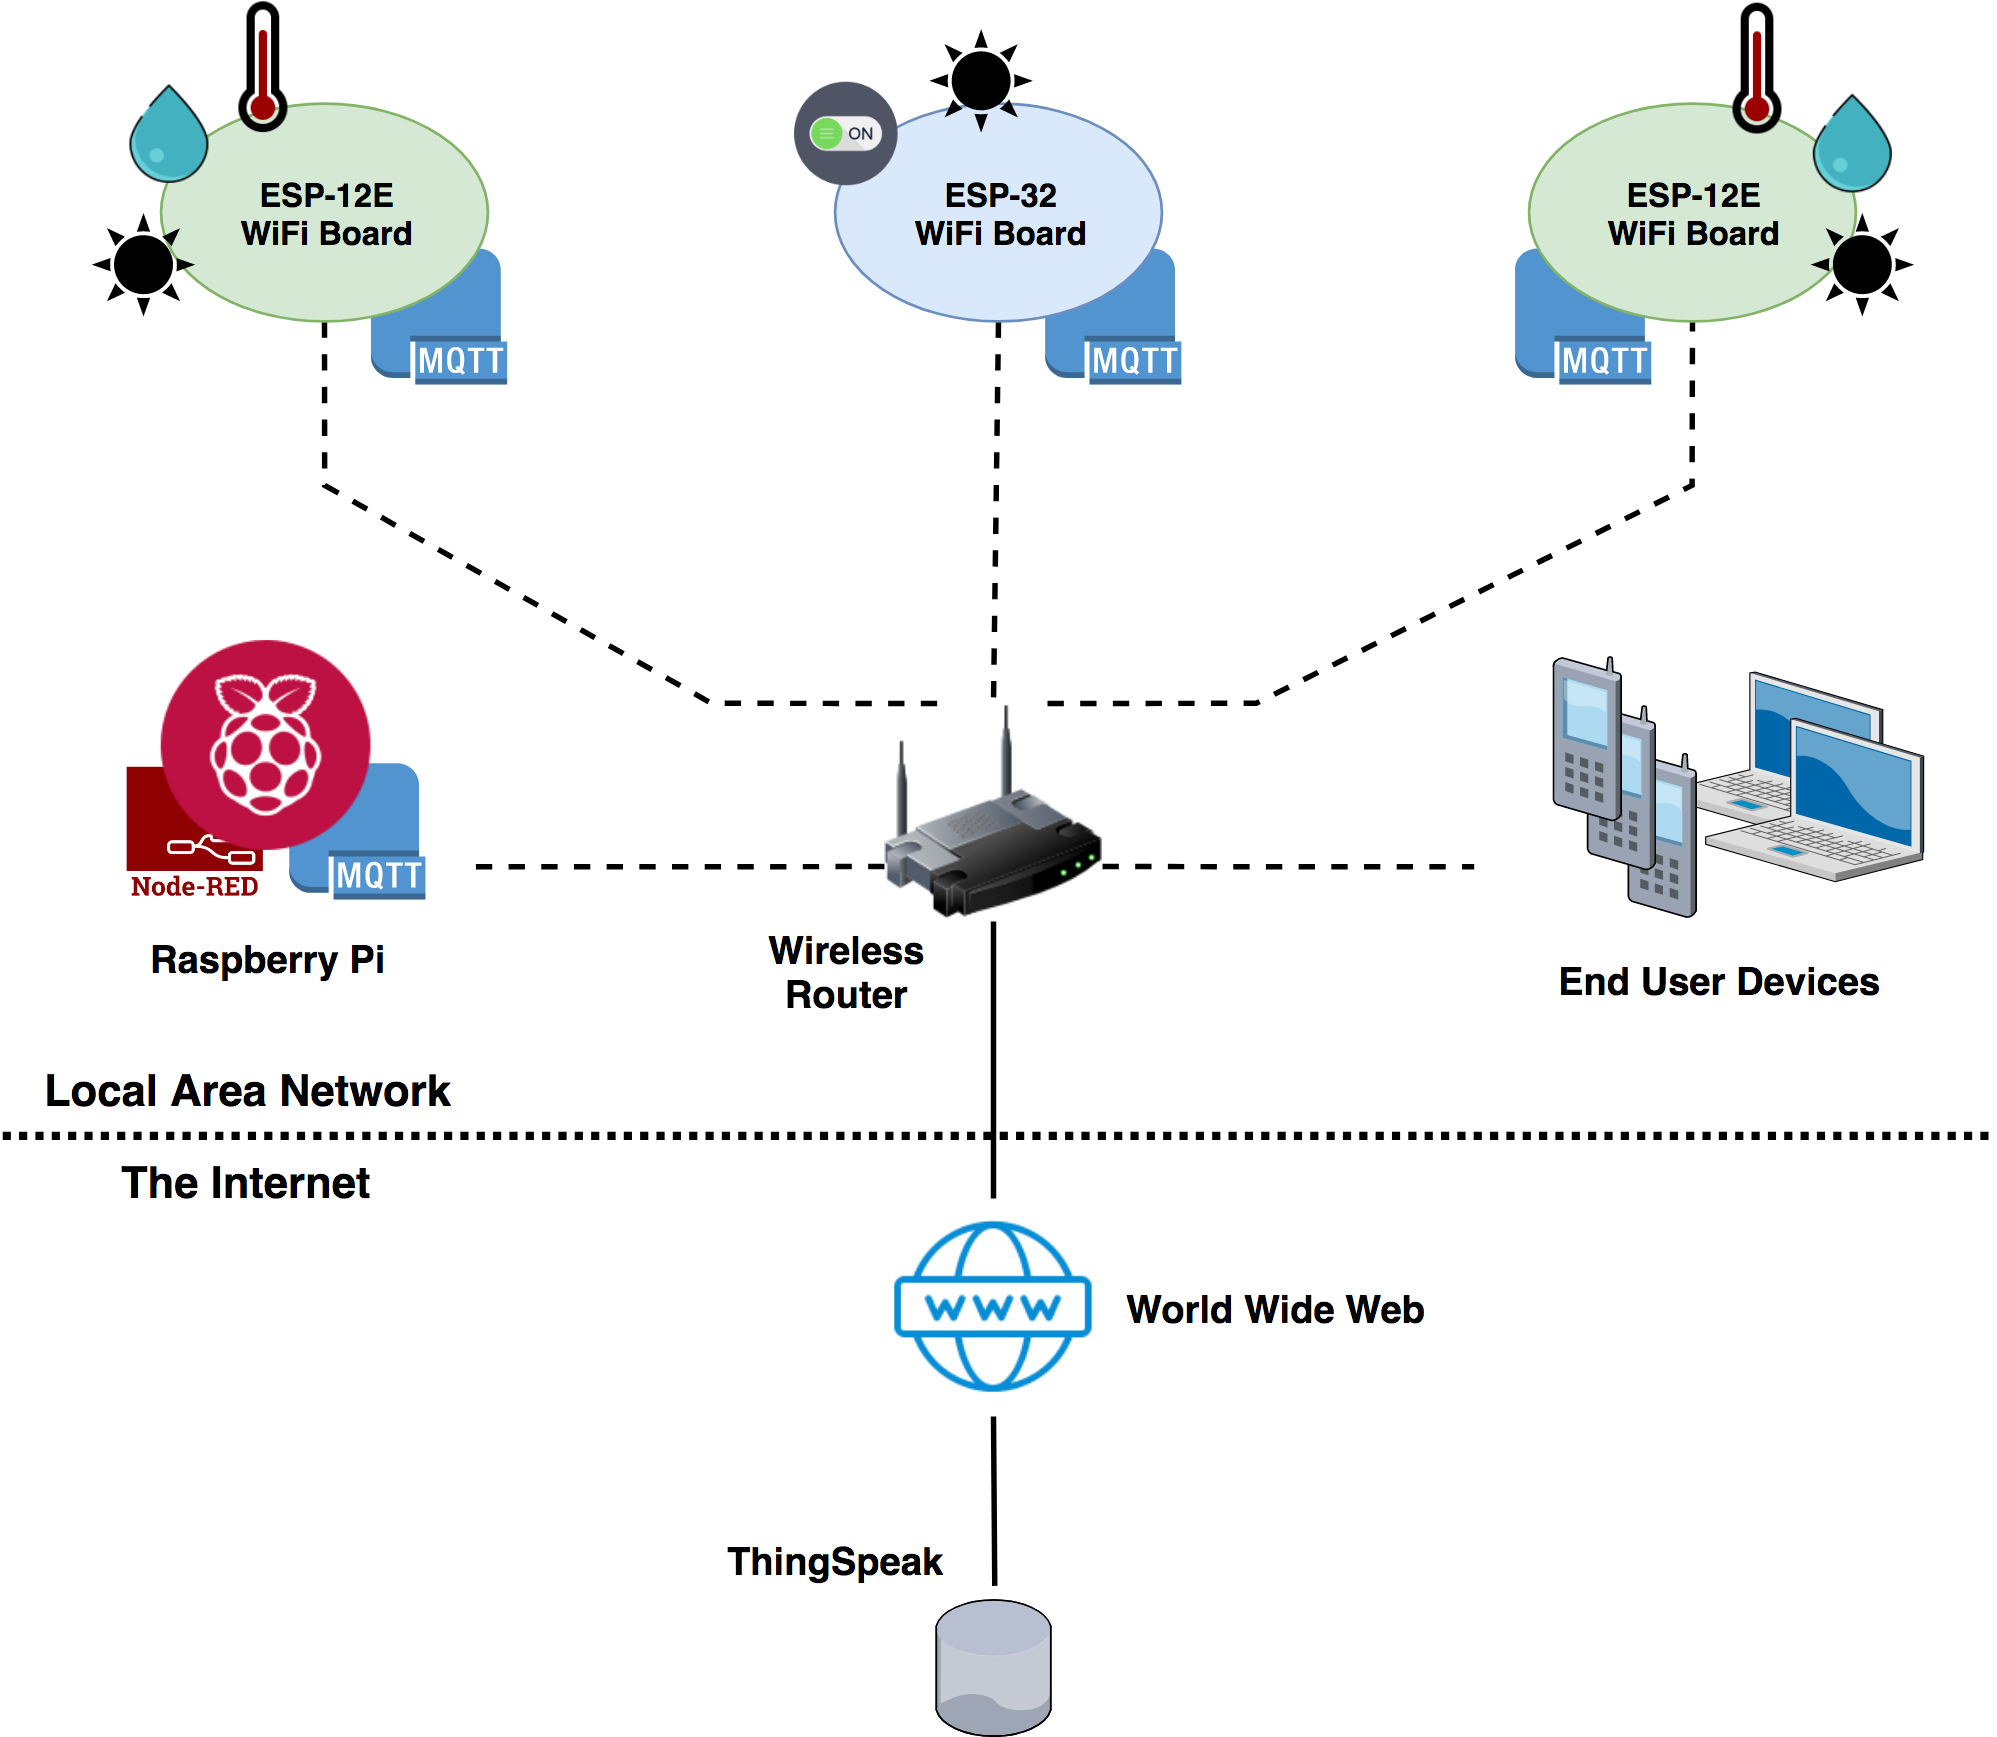
\includegraphics[width=\textwidth]{./pictures/architecture_overview.png}
		\caption{System architecture overview. Dashed lines represent wireless communication, solid lines stand for wired connections.}
		\label{architecture_overview}
	\end{center}
\end{figure}

\section{Configuring and Programming the RPi}
The Raspberry Pi is a tiny single-board computer featuring a Broadcom System-On-Chip with an integrated ARM compatible processor. There exist several different generations and models and its role in the system will suit them all. Anyway, using a Pi 3 Model B is highly recommended: it has a quad-core processor and on-board WiFi, Bluetooth and USB boot capabilities which do not require any extra module.

The Raspberry Pi board needs a fresh installation of \textit{Raspbian Stretch}, the official Debian-based Linux operating system developed by the Raspberry Pi Foundation. Other third-party operating systems are not taken into account by this document.

\begin{figure}[H]
	\begin{center}
		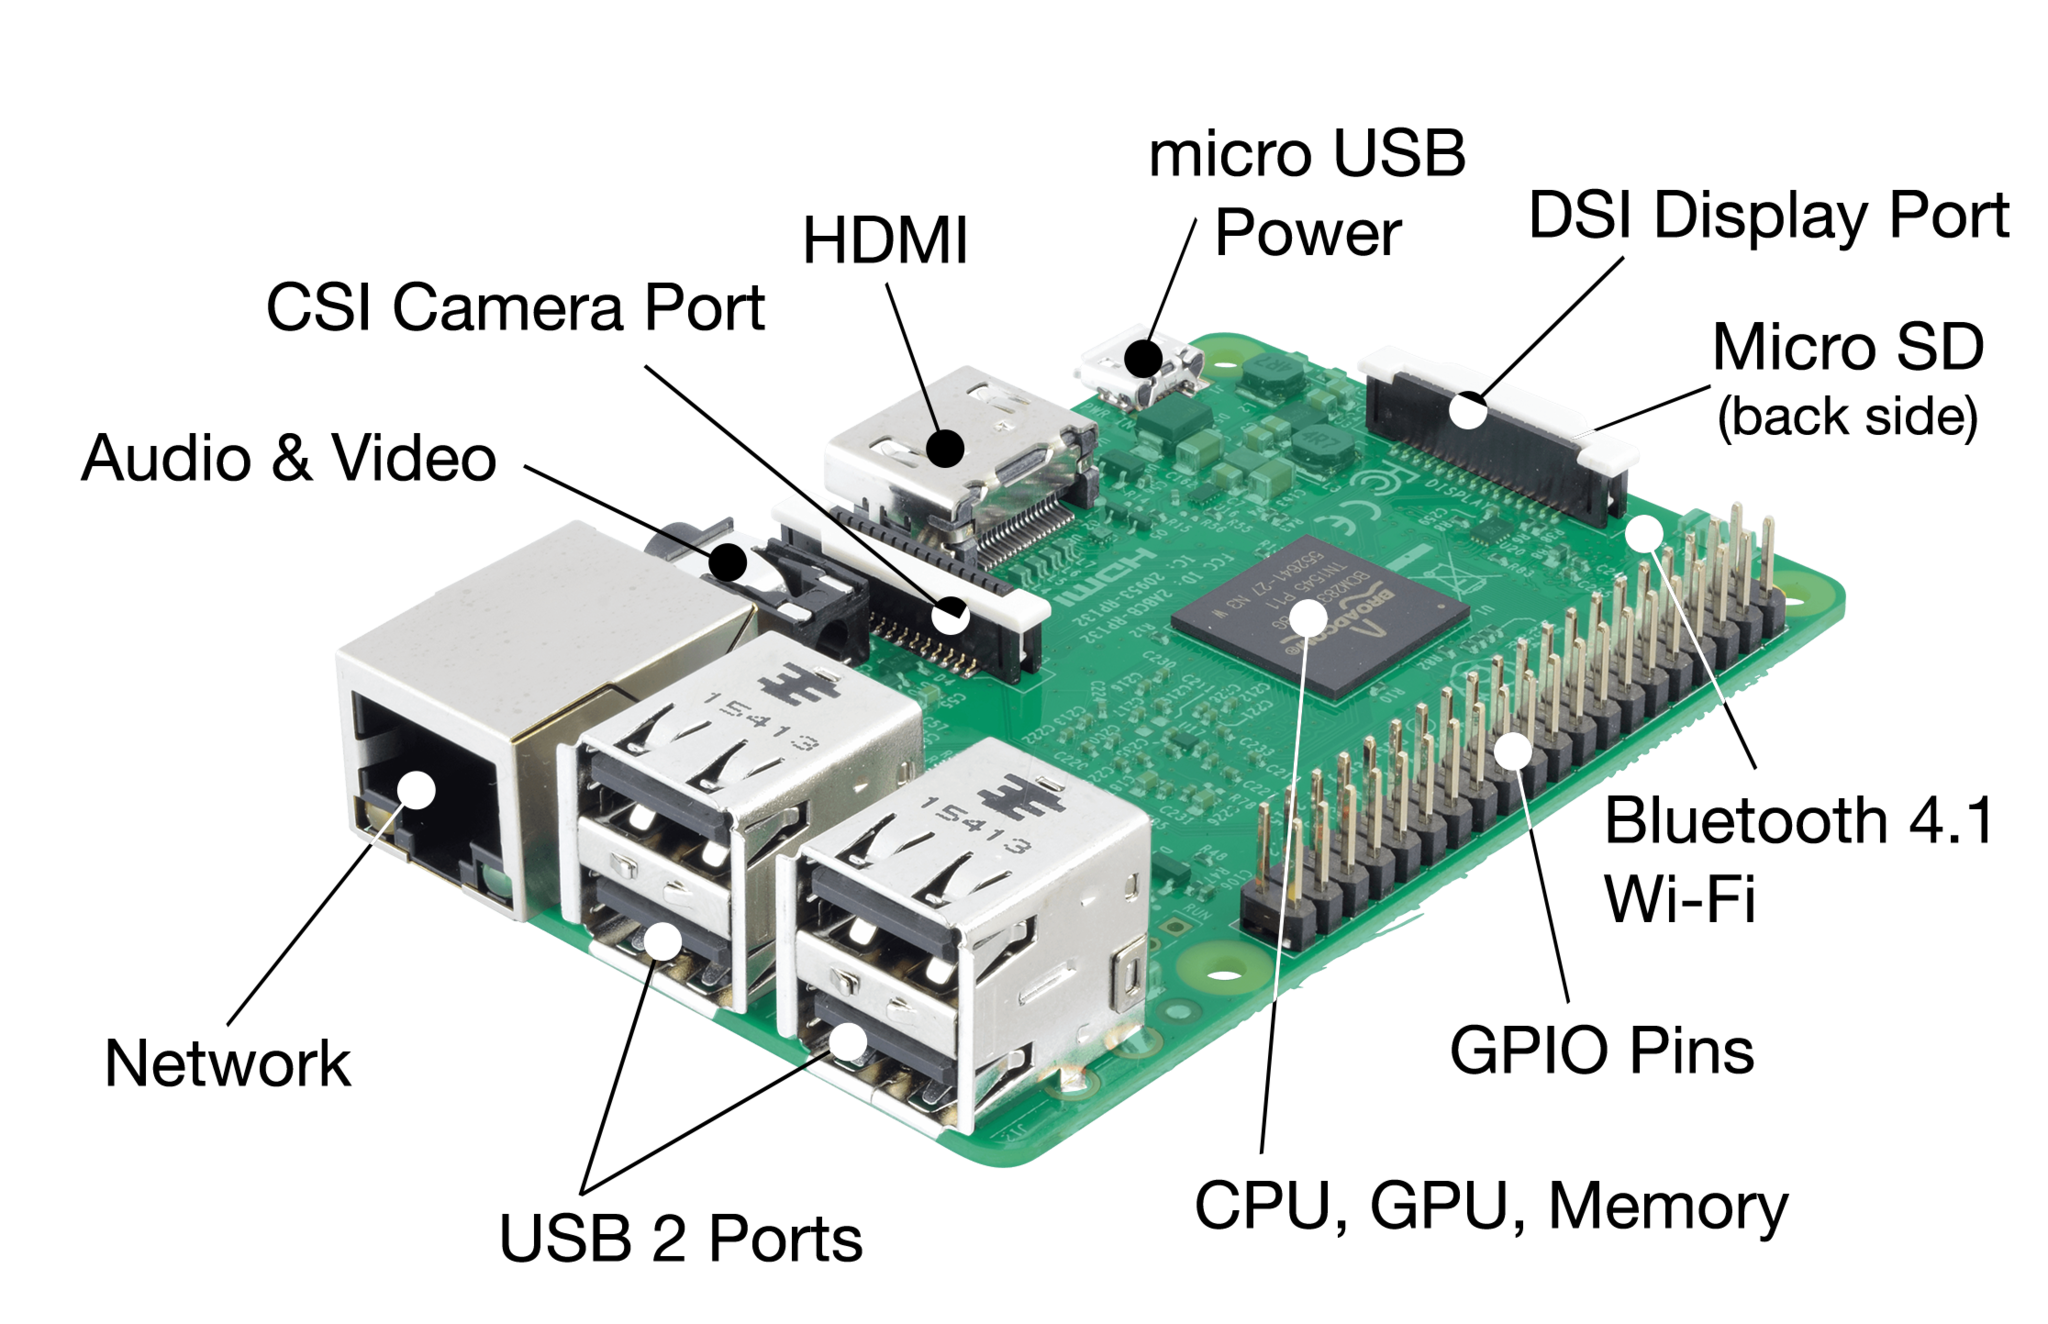
\includegraphics[width=0.6\textwidth]{./pictures/rpi_connections.png}
		\caption{Location of connectors and main integrated circuits on the Raspberry Pi 3 Model B.}
		\label{rpi_connections}
	\end{center}
\end{figure}

\noindent
The board is used as \textit{headless computer}, a device that has been configured to operate without a monitor, keyboard and mouse. The command line is accessed remotely from another computer on the same network using SSH. Since Raspbian has the SSH server disabled by default, it needs to be manually enabled from the desktop or in the terminal via \texttt{raspi-config}.

Setting up a static IP address for the Raspberry is strongly recommended. It can be assigned in the DHCP context menu of the wireless router. Since the procedure is different on any device, the router handbook should be referred to.

Before proceeding with the following sections, all the software must be up-to-date. This straightforward operation is carried out by executing the commands below in a terminal window:

\begin{verbatim}
    sudo apt-get update
    sudo apt-get upgrade
\end{verbatim}

\subsection{MQTT}
MQTT is a lightweight messaging protocol that works on top of TCP/IP. It provides resource-constrained network clients with a simple way to distribute and exchange information. MQTT is based on the publish-subscribe messaging pattern that requires a message broker to work properly: in this case the role perfectly fits the Raspberry Pi board.

Information about a given topic are sent, or published, to a server that behaves as MQTT message broker. Then, the latter pushes the information out to those clients that have previously subscribed to the above-mentioned topics.

\begin{figure}[H]
	\begin{center}
		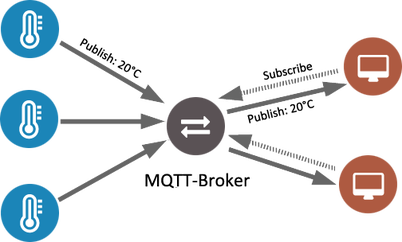
\includegraphics[width=0.6\textwidth]{./pictures/mqtt.png}
		\caption{The message broker is the central point of the MQTT infrastructure. It receives published information and forwards it to subscribed clients.}
		\label{mqtt_functioning}
	\end{center}
\end{figure}

\noindent
MQTT offers three quality of service (QoS) levels to guarantee a certain degree of performance to a data flow:

\begin{itemize}
	\item \textbf{Level 0.} At most once delivery: this is the minimal level and guarantees a best effort delivery. A message won't be acknowledged by the receiver or stored by the sender.
	\item \textbf{Level 1.} At least once delivery: all the messages will be delivered at least once to the receiver. This is the QoS level used in the \textit{Home and Automation Monitoring} system because the overhead is lower than QoS 2 and it guarantees the message arrives at least once. Duplicates are not a problem at all because the user interface would be updated one or more time with the same piece of information and this would be completely unnoticeable by the end user.
	\item \textbf{Level 2.} Exactly once delivery. It is the safest and the slowest quality of service level.
\end{itemize}

\subsection{Mosquitto}
Mosquitto is an open source message broker that implements the MQTT protocol. It is suitable for both low-power single board computers and powerful servers.

To install the broker, the following command must be run from the Raspberry Pi terminal:

\begin{verbatim}
    sudo apt-get install mosquitto
\end{verbatim}

\noindent
The broker will automatically start whenever the Raspberry is powered up. The next step is adding users and passwords to secure the MQTT connection. The current directory must be \texttt{/etc/mosquitto} while typing the successive commands:

\begin{verbatim}
    // Add the first user
    sudo mosquitto_passwd -c passwordfile user
    
    // Add another user to the existing password file
    sudo mosquitto_passwd -b passwordfile other_user password
\end{verbatim}

\noindent
The following two lines must be added to the \texttt{mosquitto.conf} file.

\begin{verbatim}
    allow_anonymous false
    password_file /etc/mosquitto/passwordfile
\end{verbatim}

\noindent
As far as this system is concerned, just a single user has been created to manage the MQTT connection: username is \texttt{admin} and password is \texttt{hamrpi}. These credentials are used to set up MQTT by Node-RED and any ESP node.

\subsection{Node-RED}

\subsubsection{Description}
Node-RED is a programming tool for wiring together hardware devices, APIs and online services in new and interesting ways.
It provices a browser-based editor that makes it easy to wire together flows using the wide range of nodes in the palette that can be deployed to its runtime in a single-click.

\subsubsection{Installation}
Node-RED comes preinstalled on the full Raspbian SD card image that can be donwloaded from RaspberryPi.org.

\noindent
If you have a version of Raspbian, or other Debian based install, such as Ubuntu, or Diet-Pi, that doesn't have Node-RED already installed, you can install or upgrade using the Node-RED upgrade script command:

\begin{verbatim}
bash <(curl -sL https://raw.githubusercontent.com/node-red
/raspbian-deb-package/master/resources/update-nodejs-and-nodered)>
\end{verbatim}

\noindent
It is also necessary to install another node component to manage the secure access of node-red.
\newline
\newline
From the Raspberry Pi it is needed to run the following commands:
\begin{verbatim}
cd ~/.node-red
sudo npm install -g node-red-admin
\end{verbatim}

\noindent
Finally inside node-red it is necessary to install a plugin to manage the connection with the Raspberry Pi through the MQTT protocol.
\newline
\newline
Inside the settings of Node-red, you go to Manage Pallette and install the plugin:
\begin{verbatim}
node-red-bashboard
\end{verbatim}
\begin{figure}[H]
	\begin{center}
		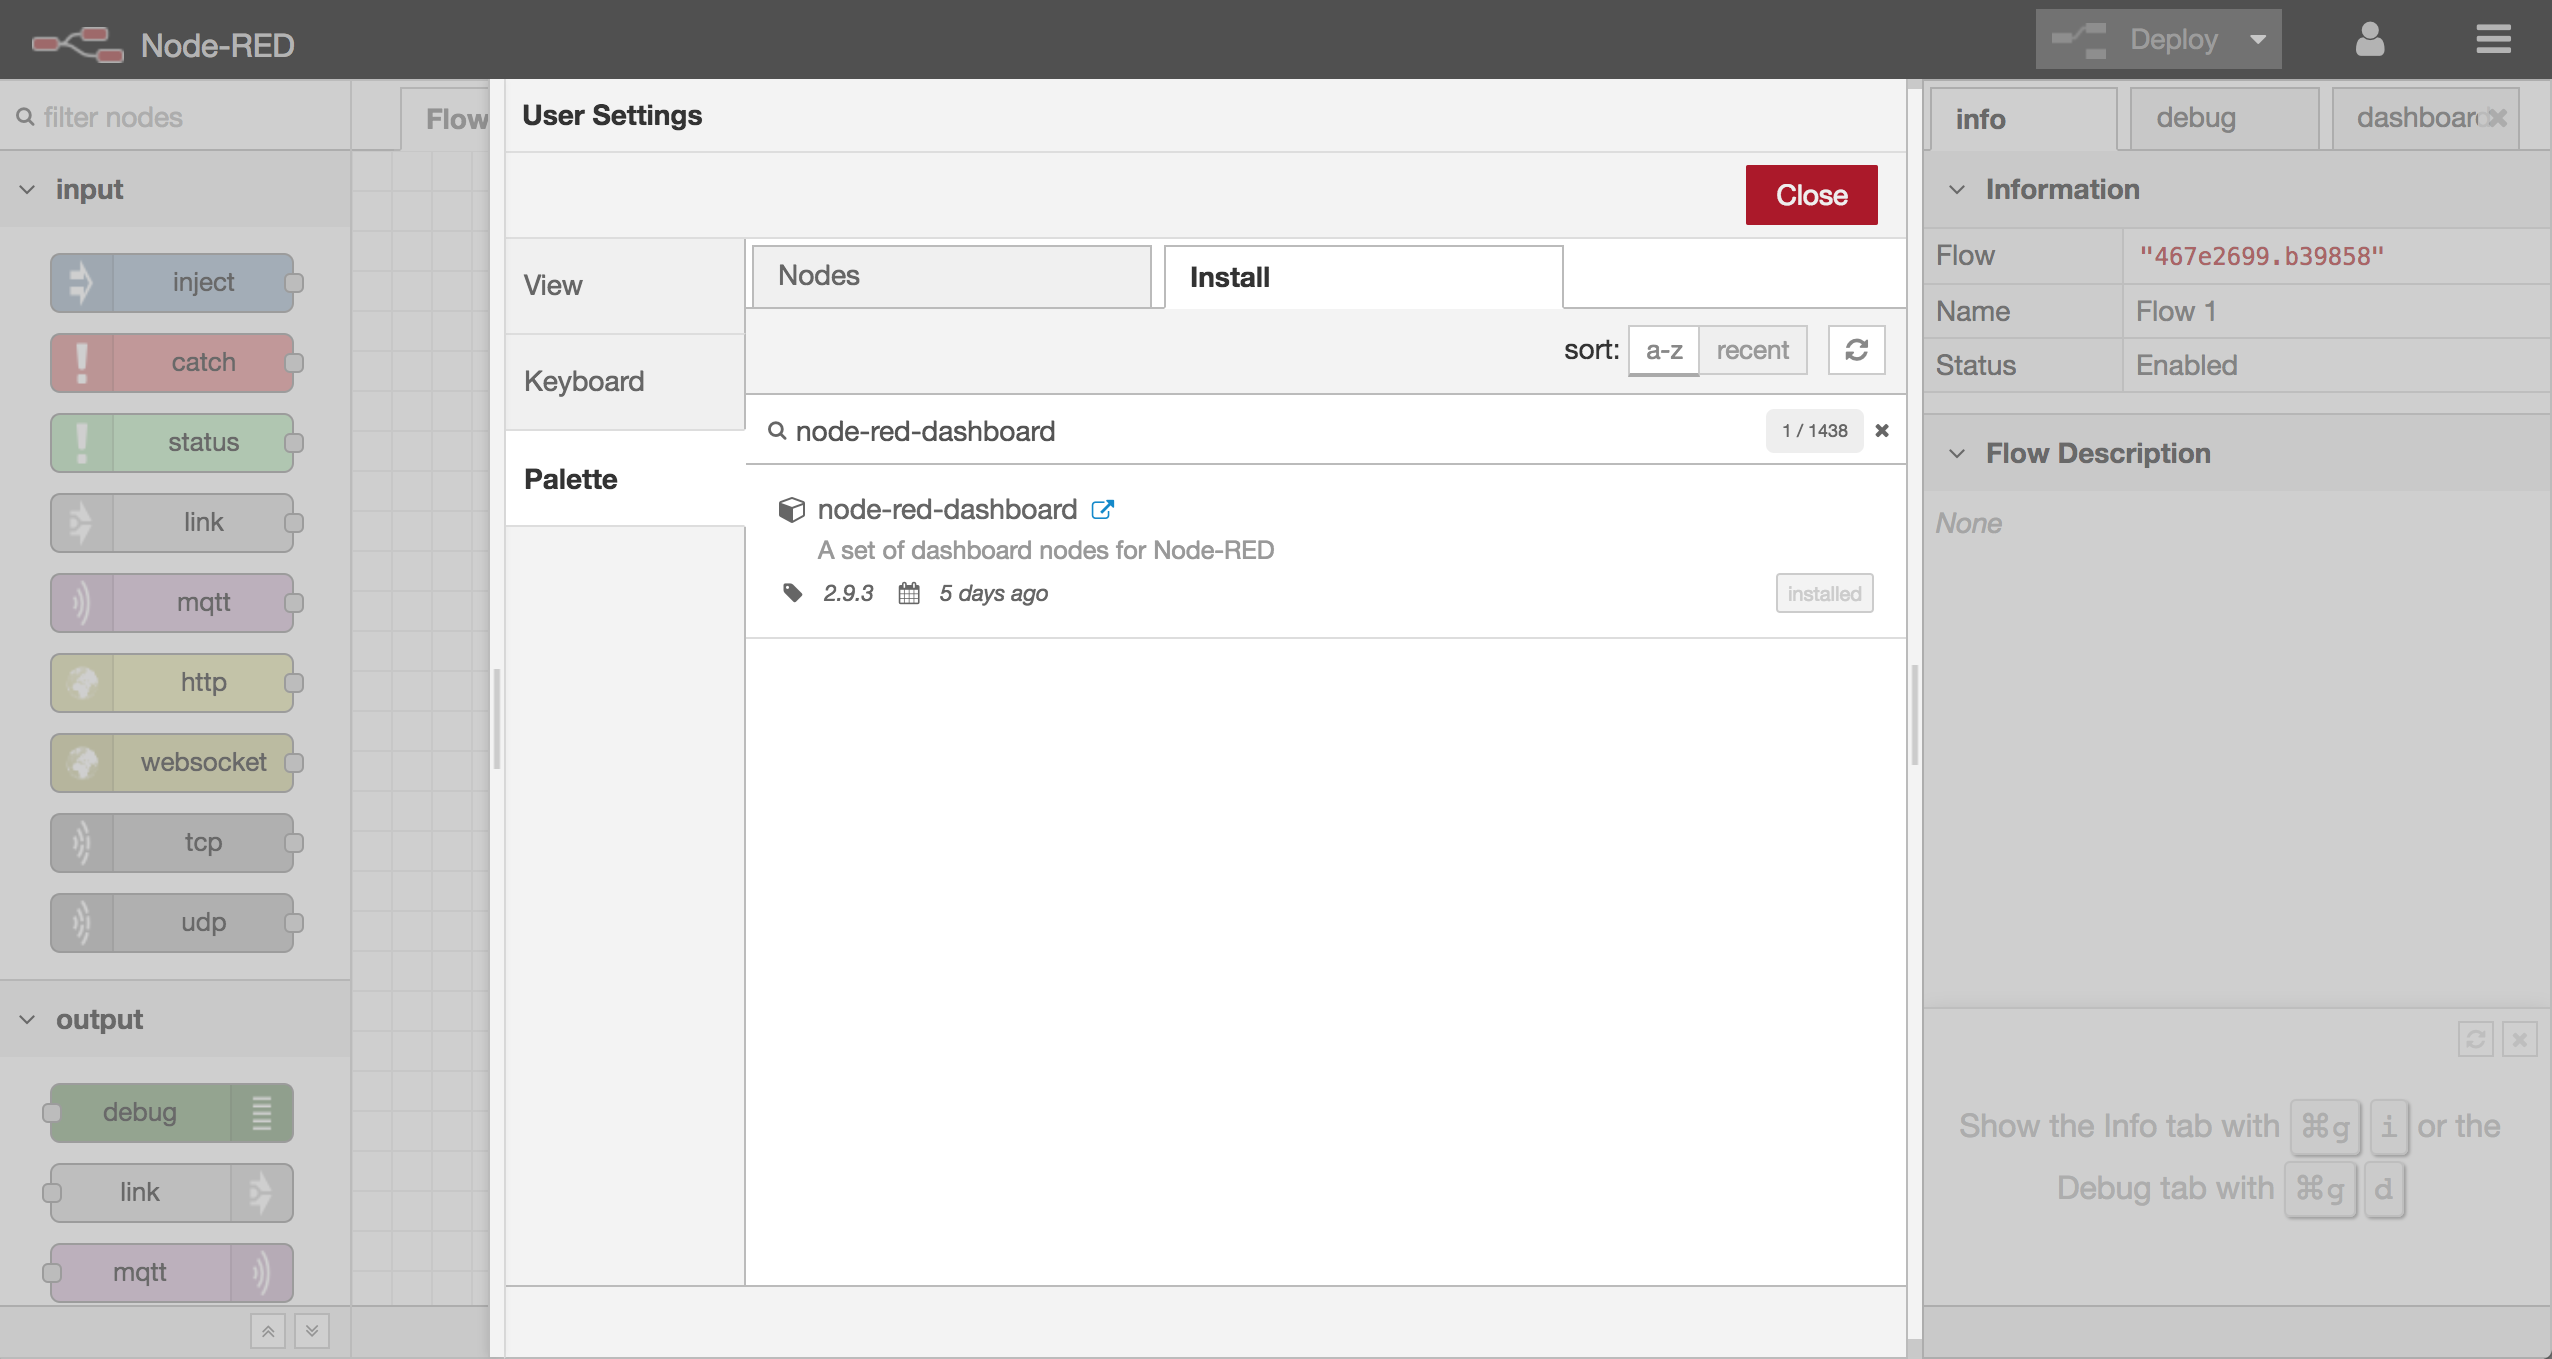
\includegraphics[width=1.0\textwidth]{./pictures/node-red-dashboard}
		\caption{Node-Red Manage Pallette UI}
		\label{mqtt_functioning}
	\end{center}
\end{figure}

\subsubsection{Access Control}
The following tasks must be performed from a terminal ssh session towards the Raspberry Pi.
\newline
You have to enable the secure access to node-red, setting an admin username and password, and it is also possibile to add other users with a different permissions.
\newline
\newline
The first step is to generate the hash of the admin password, that'll be saved in the configuration file of node-red ''setting.js'', simply running the following command:
\begin{verbatim}
node-red-admin hash-pw
\end{verbatim}
After that we insert the chosen password and as a result we get the hash of the password.

\begin{figure}[H]
	\begin{center}
		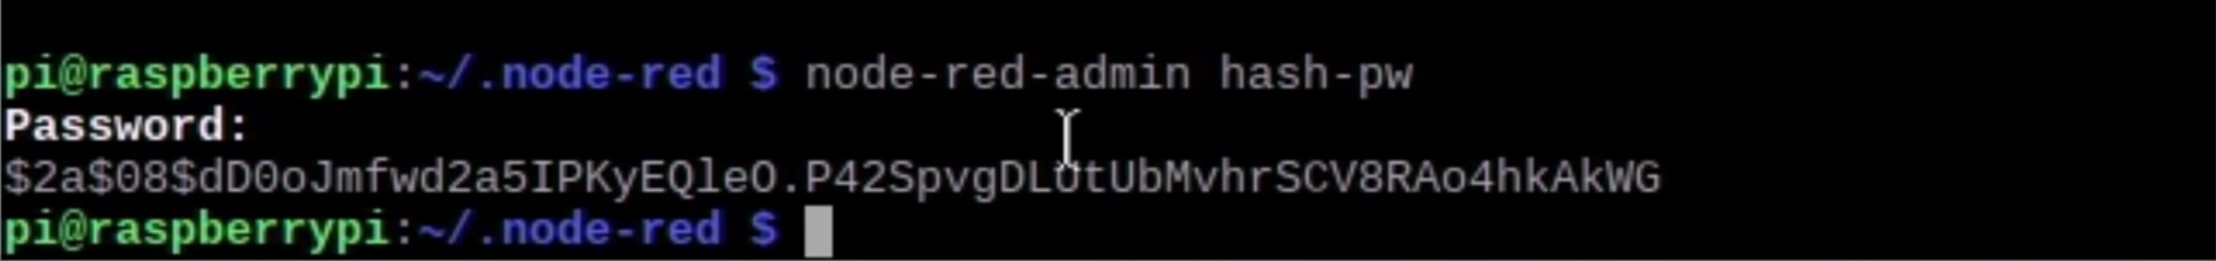
\includegraphics[width=1.0\textwidth]{./pictures/node-red_hash_password}
		\caption{Node-Red hash password generation example}
		\label{mqtt_functioning}
	\end{center}
\end{figure}

\noindent
The second step is to modify the configuration file ''settings.js'' of node-red.
\newline
The file is located usually at the following path
\begin{verbatim}
cd ~/.node-red
\end{verbatim}
Then open the file \emph{settings.js} with nano or vim.
\begin{verbatim}
vim settings.js
\end{verbatim}
At this point we need to change the file as depicted in the image below.

\begin{figure}[H]
	\begin{center}
		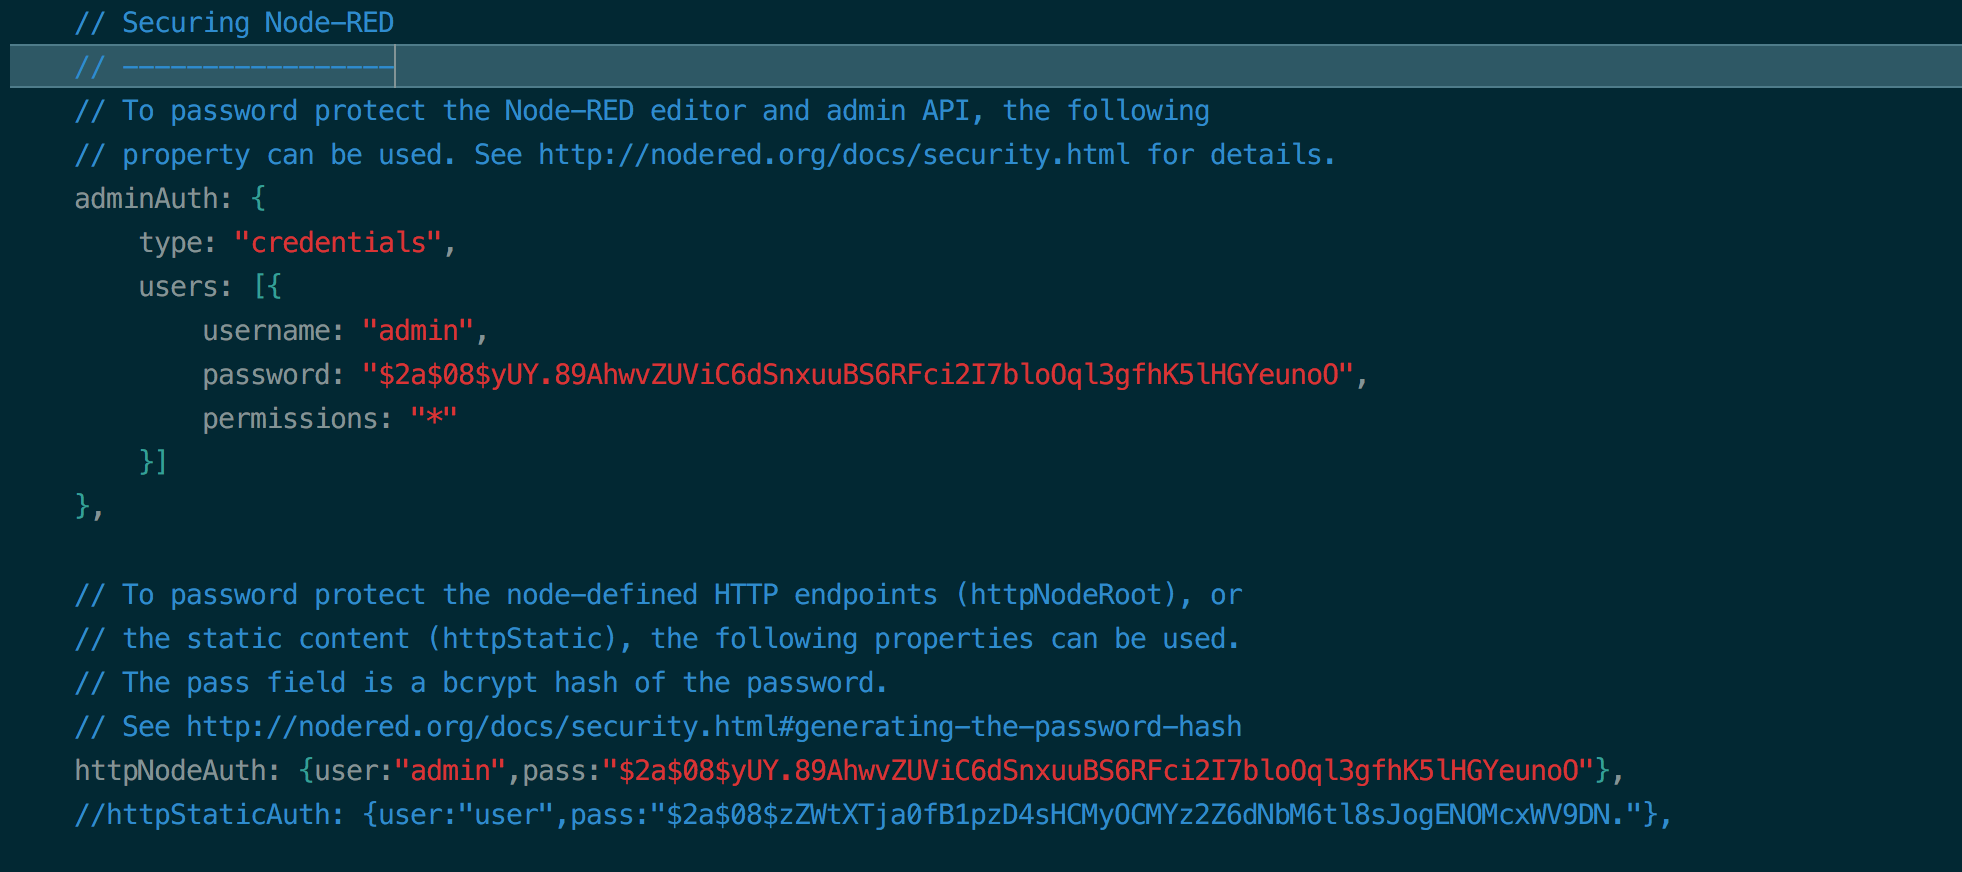
\includegraphics[width=1.0\textwidth]{./pictures/node-red-secure}
		\caption{Node-Red config file setting.js secure access enabling}
		\label{mqtt_functioning}
	\end{center}
\end{figure}

\noindent
As final step you have to restart the node-red service such that when you switch-on the Raspberry Pi node-red automatically starts.
\newline
This feature is activated running the following code:
\begin{verbatim}
sudo systemctl enable nodered.service
reboot
\end{verbatim}
Note that you have to reboot the system after the previous modifications.
\newline
\newline
After the system is restarted if you try to connect to the node-red URL, you should have something like what depicted below: 

\begin{figure}[H]
	\begin{center}
		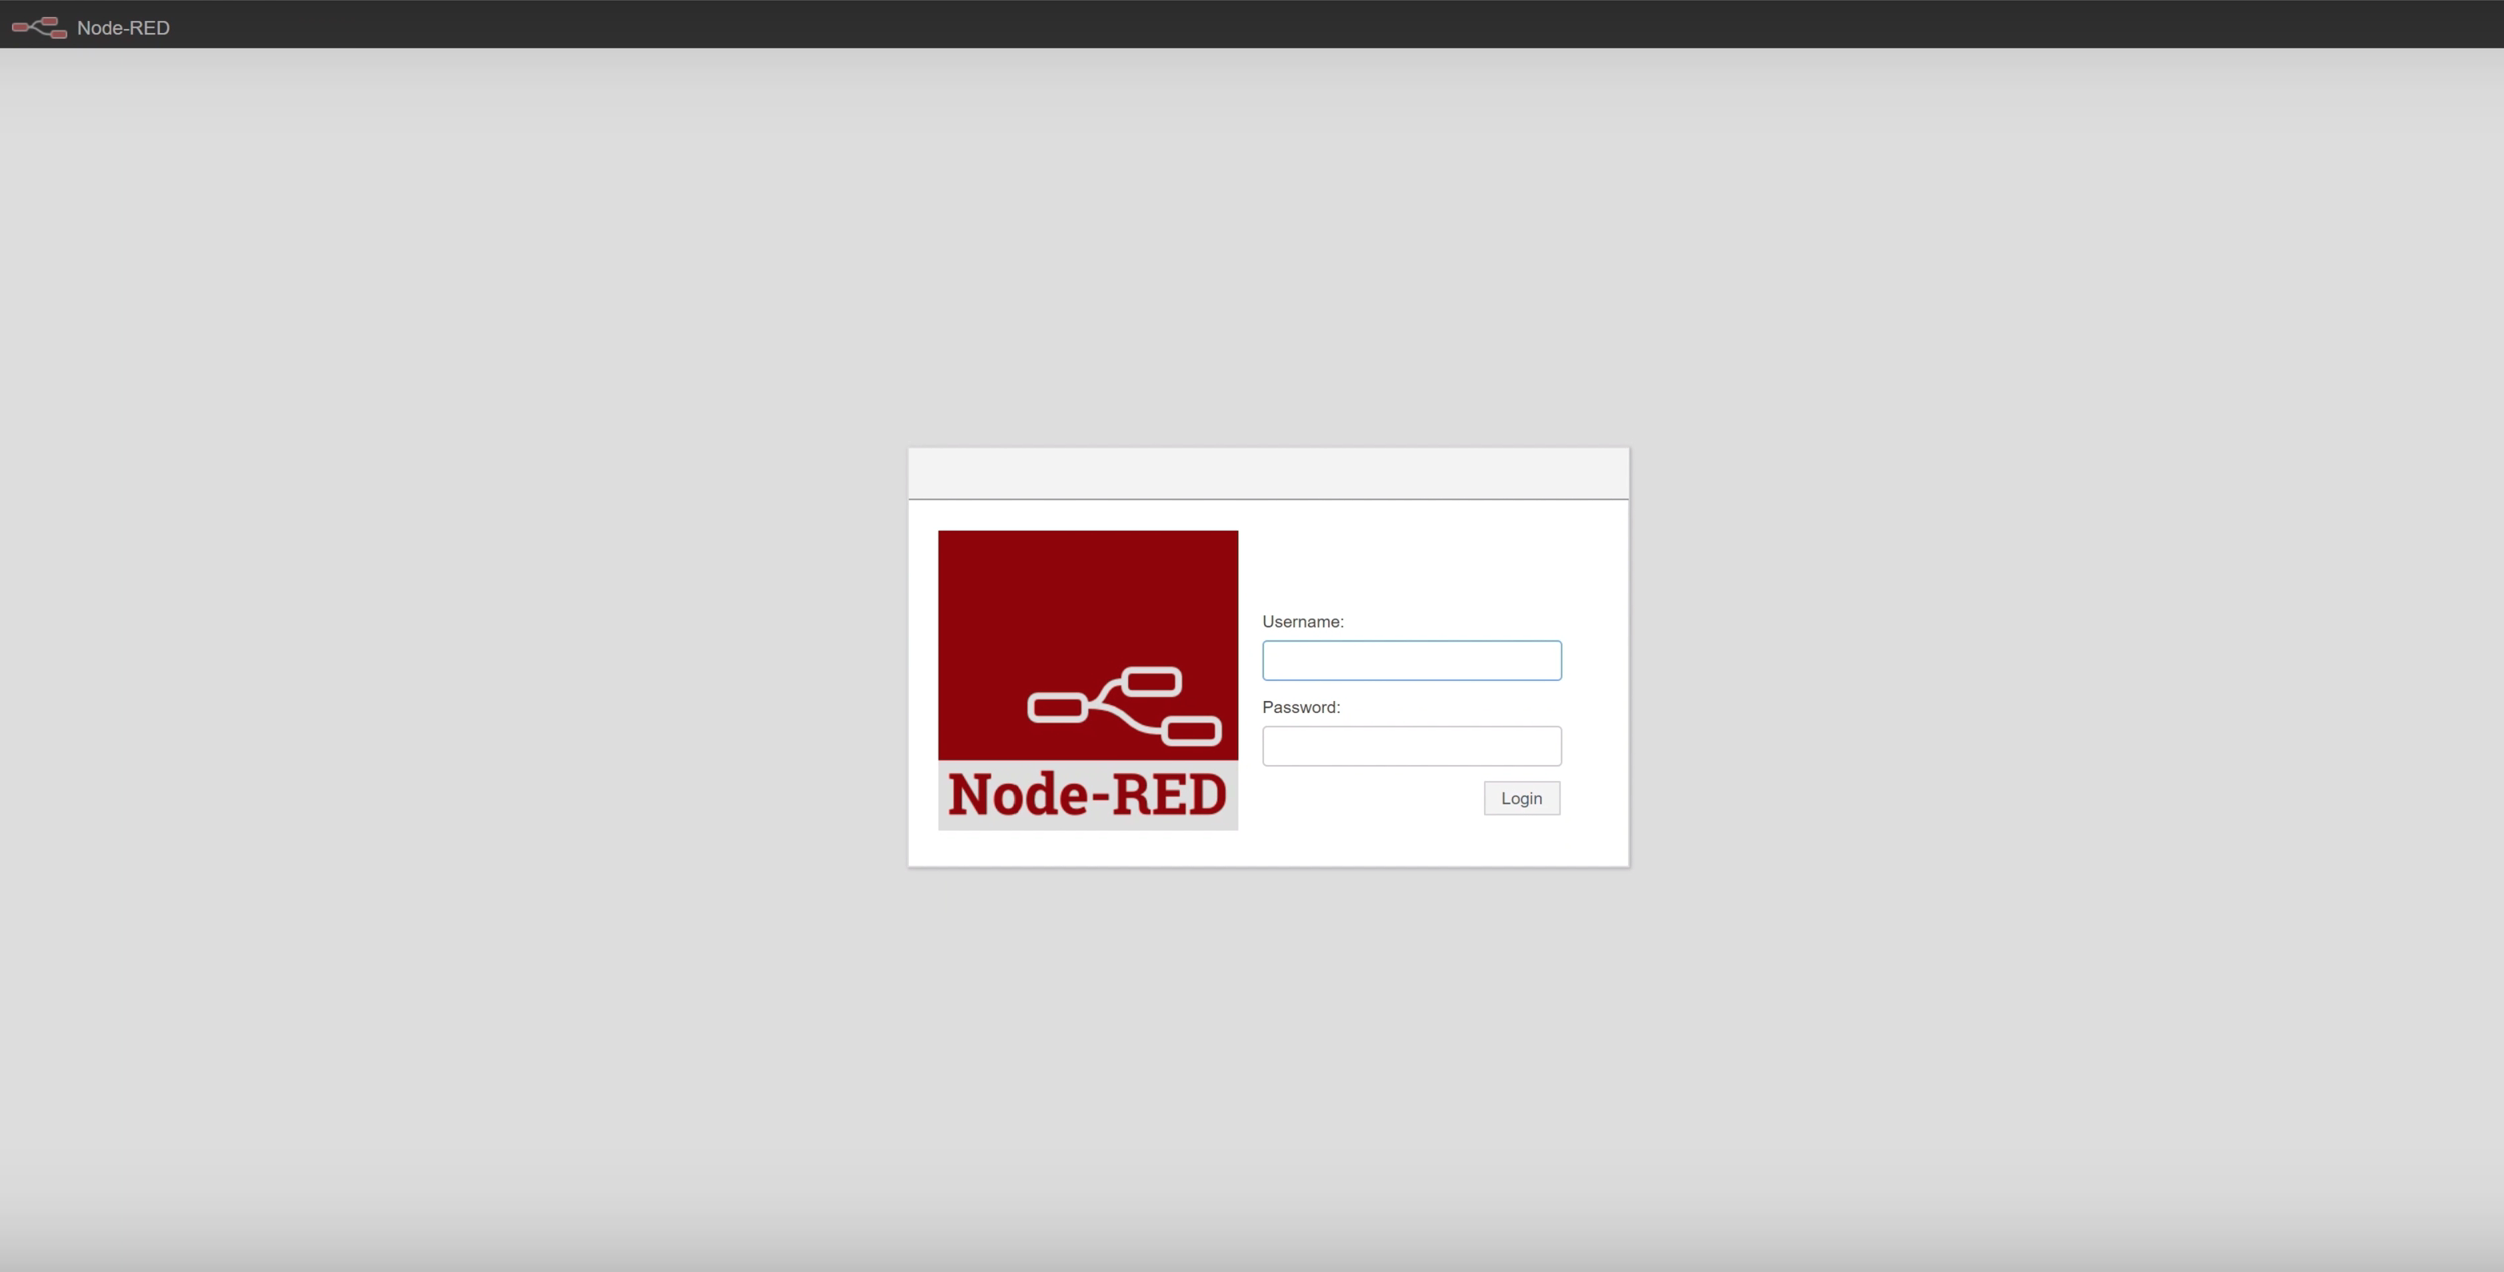
\includegraphics[width=1.0\textwidth]{./pictures/node-red-UI-login}
		\caption{Node-Red UI login}
		\label{mqtt_functioning}
	\end{center}
\end{figure}



\subsubsection{Main Block Nodes}
The nodes used for the UI of the dashboard are the followings:
\begin{itemize}
    \item \textbf{MQTT}: taken from the input and also output nodes menu.\\
    This node is used to manage the connection with the Mqtt broker installed in the Raspberry PI to get the data based on the subscriptions of the nodes.
    \item \textbf{GAUGE}: taken from the dashboard nodes menu.\\
    This node allows to display the current value measured from a certain sensor with different types of representation (i.e. gauge, donut, compass or level) in the dashboard UI.
    \item \textbf{CHART}: taken from the dashboard nodes menu.\\
    This node is used to show the most recent data captured by the motes into the dashboard UI.
    \item \textbf{SWITCH}: taken from the dashboard nodes menu.\\
    This node is responsible for managing the status of the relay that one of the motes is equipped with.
\end{itemize}

\subsubsection{Dashboard UI}
The dashboard looks like this:

\begin{figure}[H]
	\begin{center}
		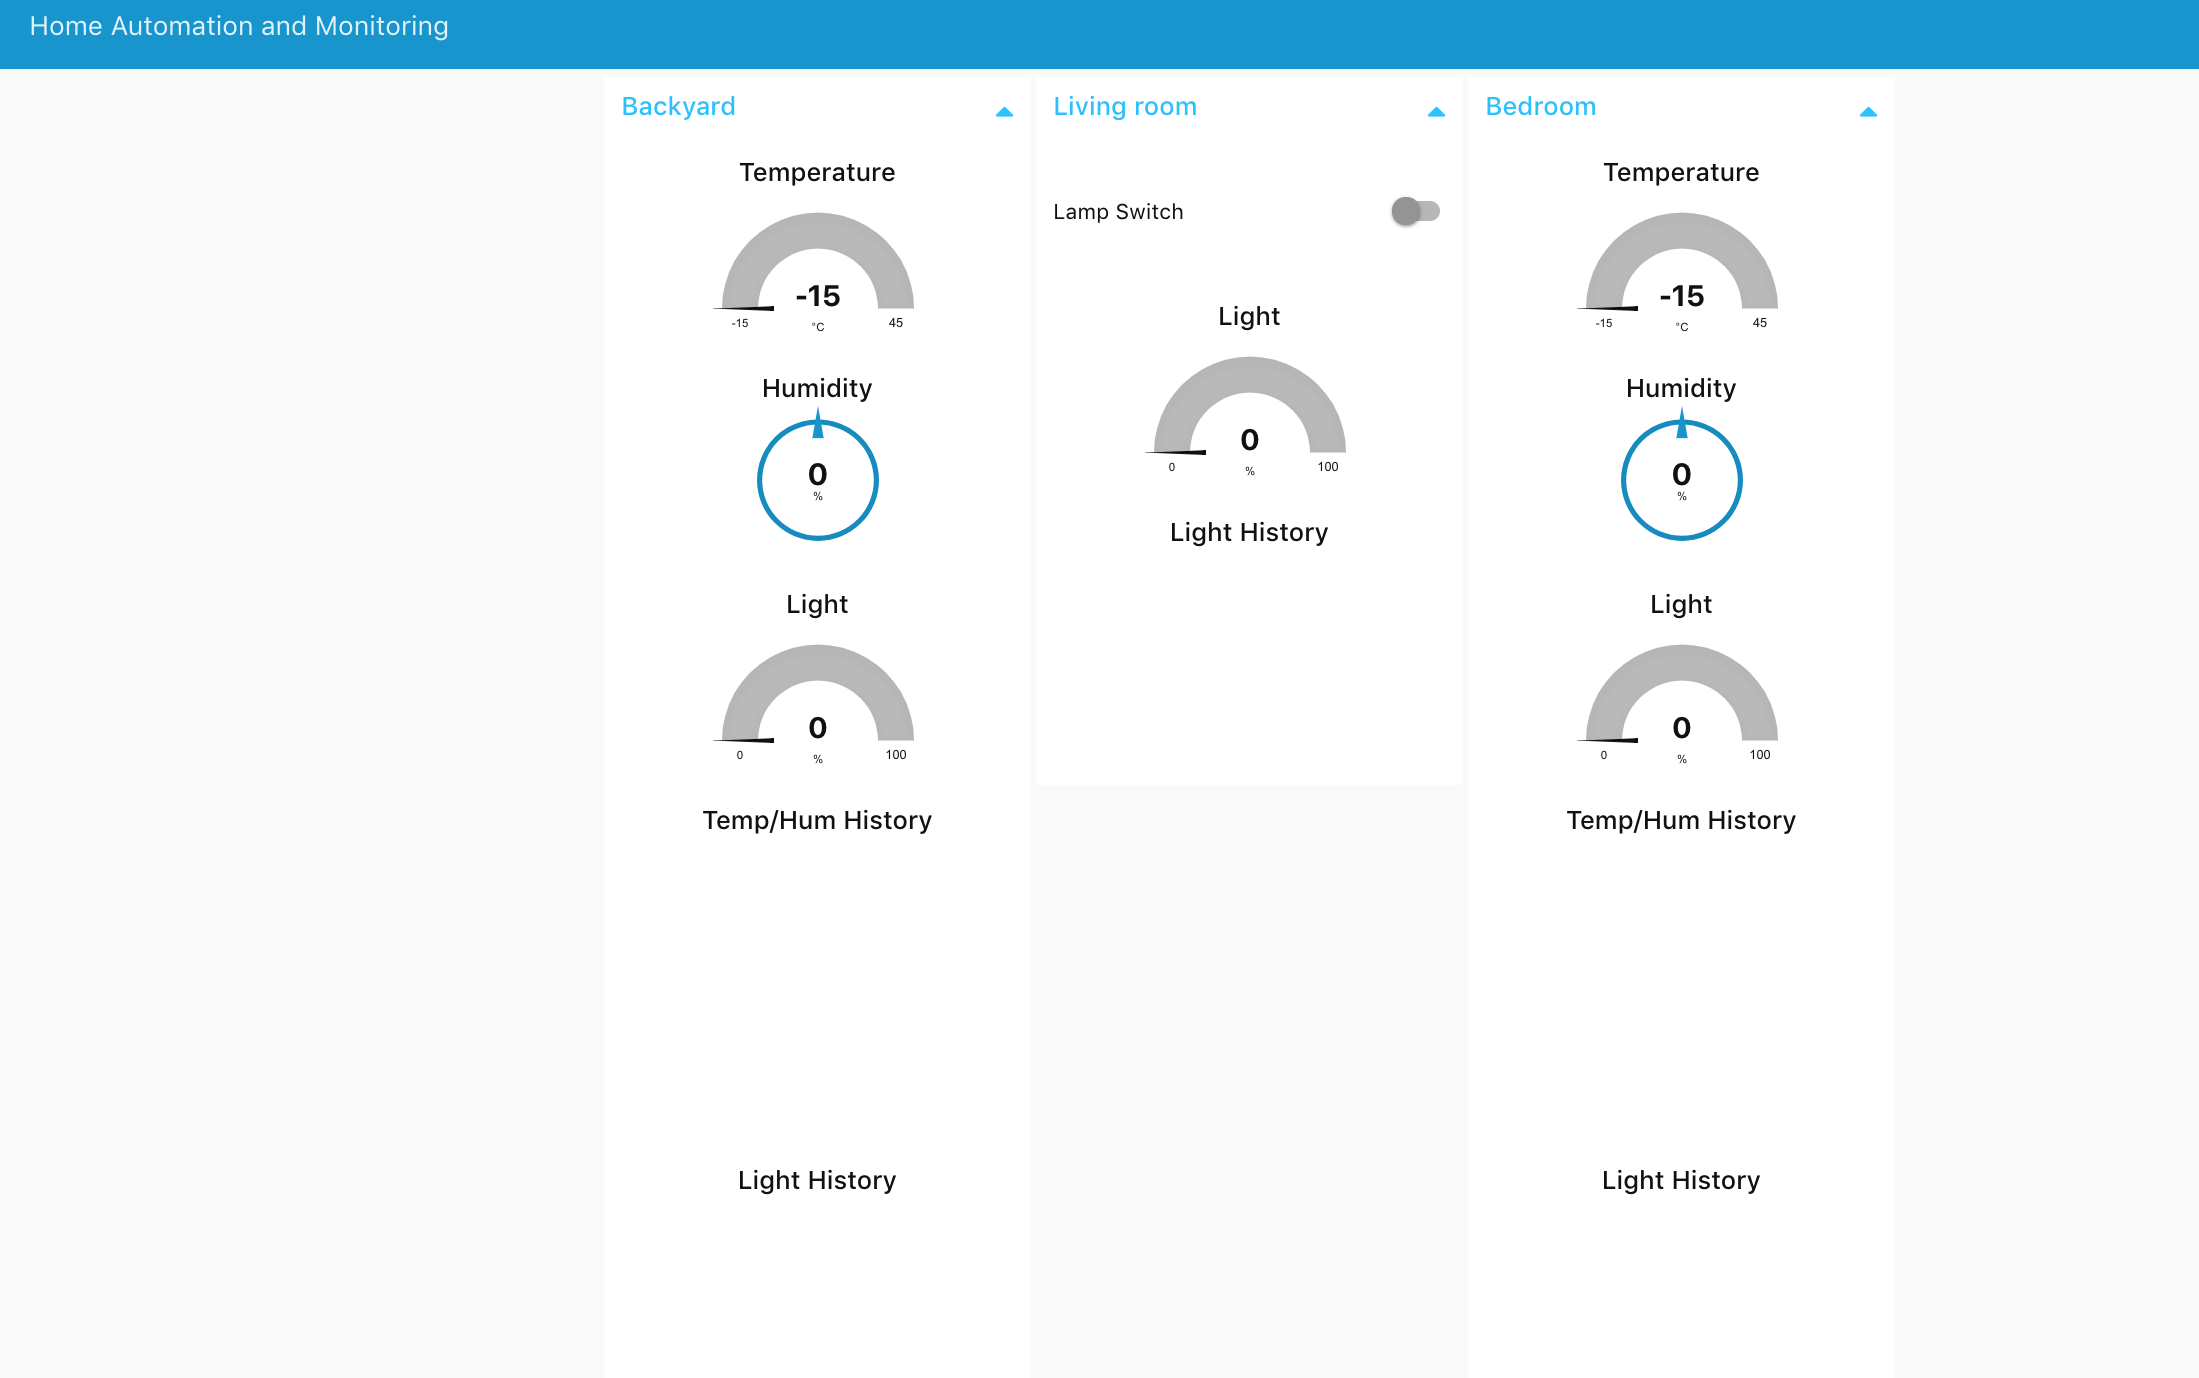
\includegraphics[width=1.0\textwidth]{./pictures/laptop_dashboard}
		\caption{Node-Red dashboard laptop UI}
		\label{mqtt_functioning}
	\end{center}
\end{figure}

\begin{figure}[H]
	\begin{center}
		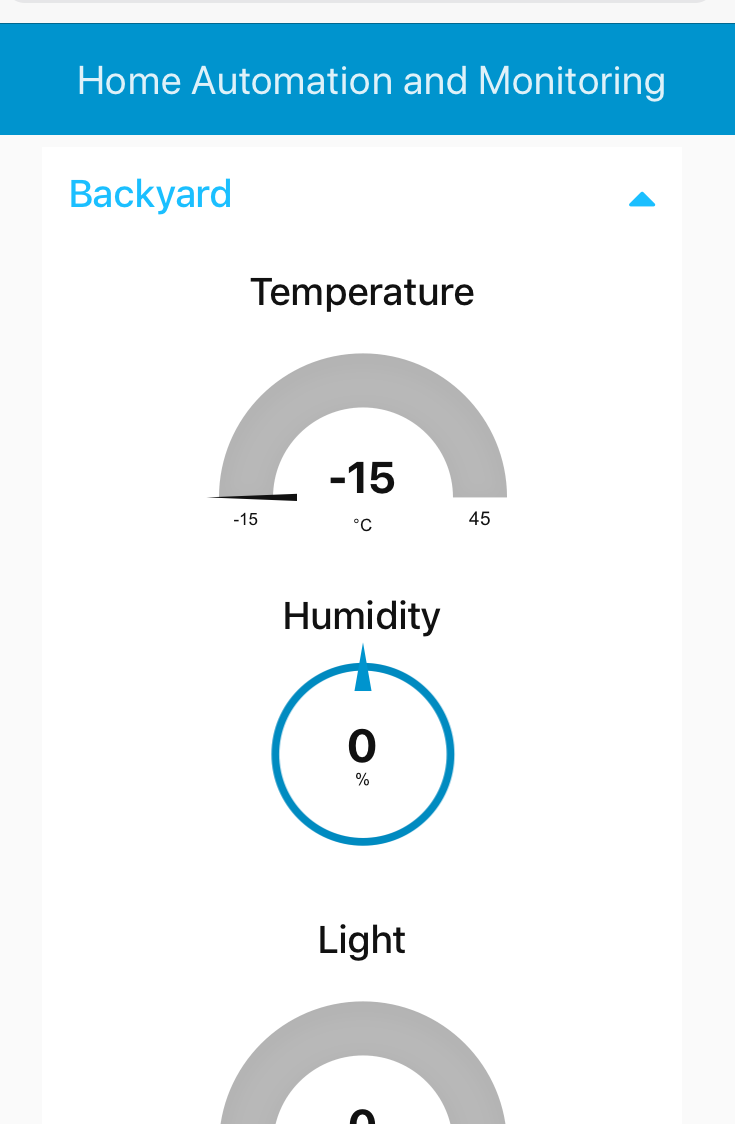
\includegraphics[width=0.3\textwidth]{./pictures/smartphone_dashboard.PNG}
		\caption{Node-Red dashboard smartphone UI}
		\label{mqtt_functioning}
	\end{center}
\end{figure}

\subsection{ThingSpeak}

\subsubsection{Description}
ThingSpeak  is an IoT platform that lets you collect and store sensor data in the cloud and develop IoT applications. The ThingSpeak IoT platform provides apps that let you analyze and visualize your data in MATLAB, and then act on the data. Sensor data can be sent to ThingSpeak from Arduino, Raspberry Pi, BeagleBone Black, and other hardware.

\subsubsection{Channel setup}
Once logged on ThingSpeak you have to create a new channel and set it up in the following way.

\begin{figure}[H]
	\begin{center}
		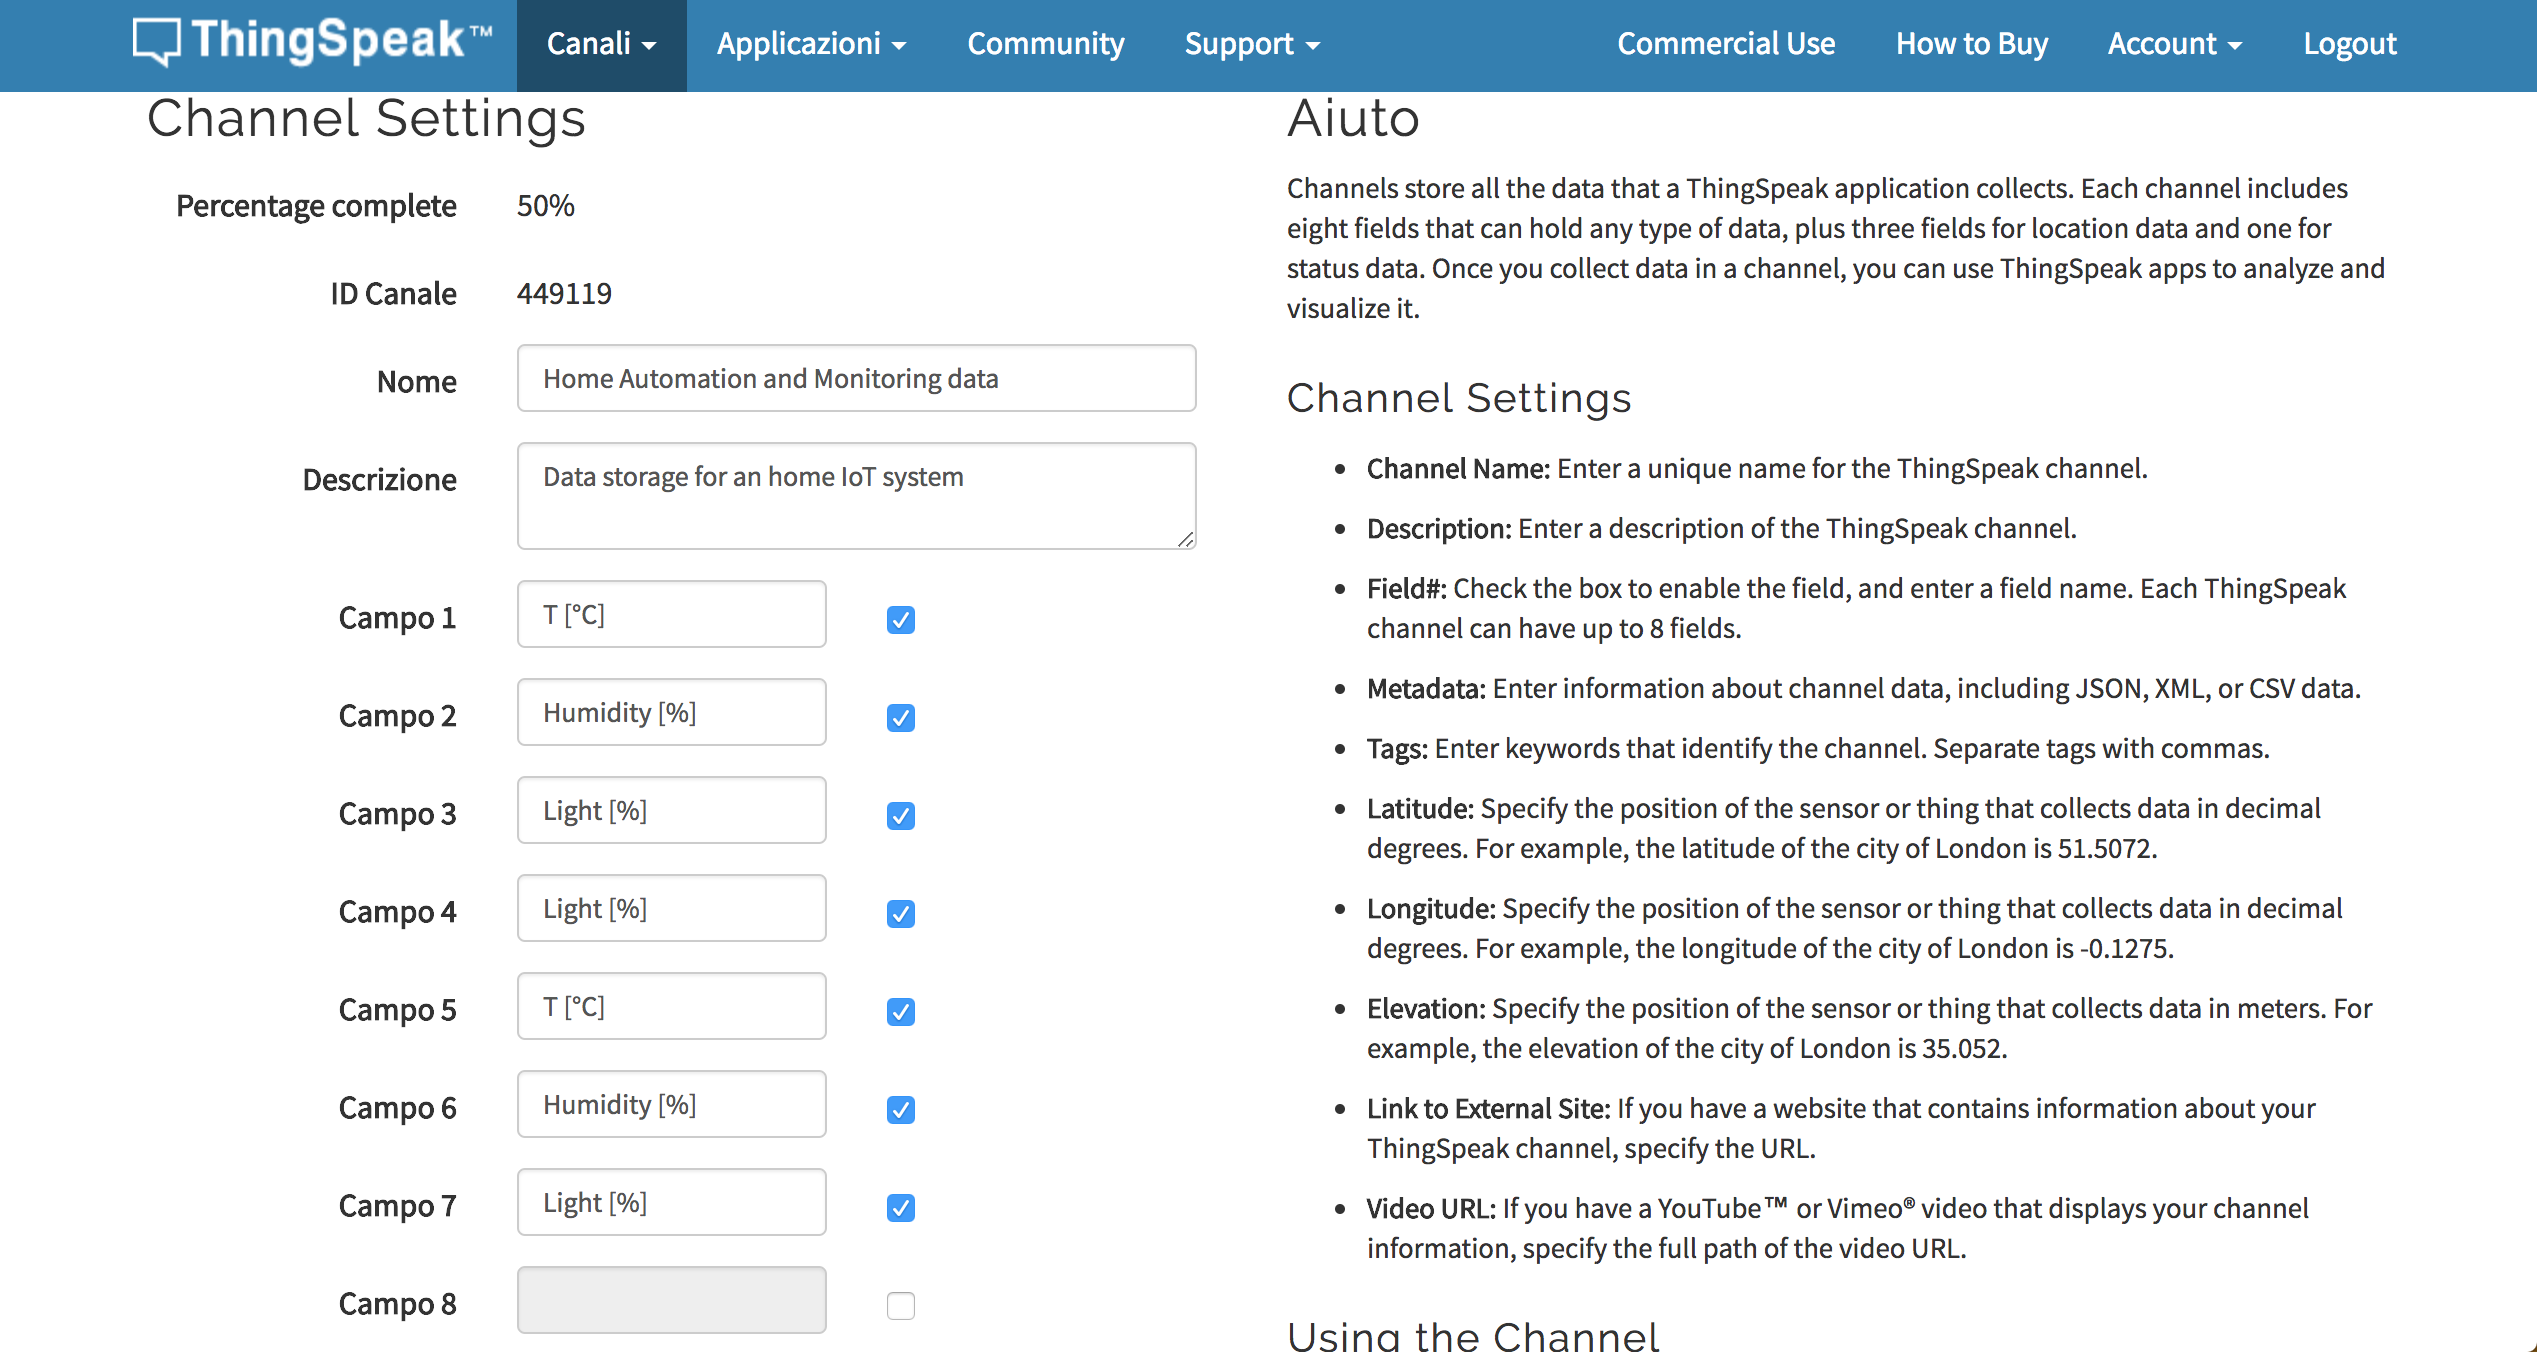
\includegraphics[width=0.8\textwidth]{./pictures/thingspeak-channels-setup}
		\caption{ThingSpeak channels setup}
		\label{mqtt_functioning}
	\end{center}
\end{figure}

\noindent
Every field is linked to a different sensor of a mote and collects all the data that receives from it.
\newline
\newline
After this you need to copy the API Key that is used to send data to ThingSpeak from Node-Red.
\newline
In particular you have to copy the \emph{Update a Channel Feed} Url.

\begin{figure}[H]
	\begin{center}
		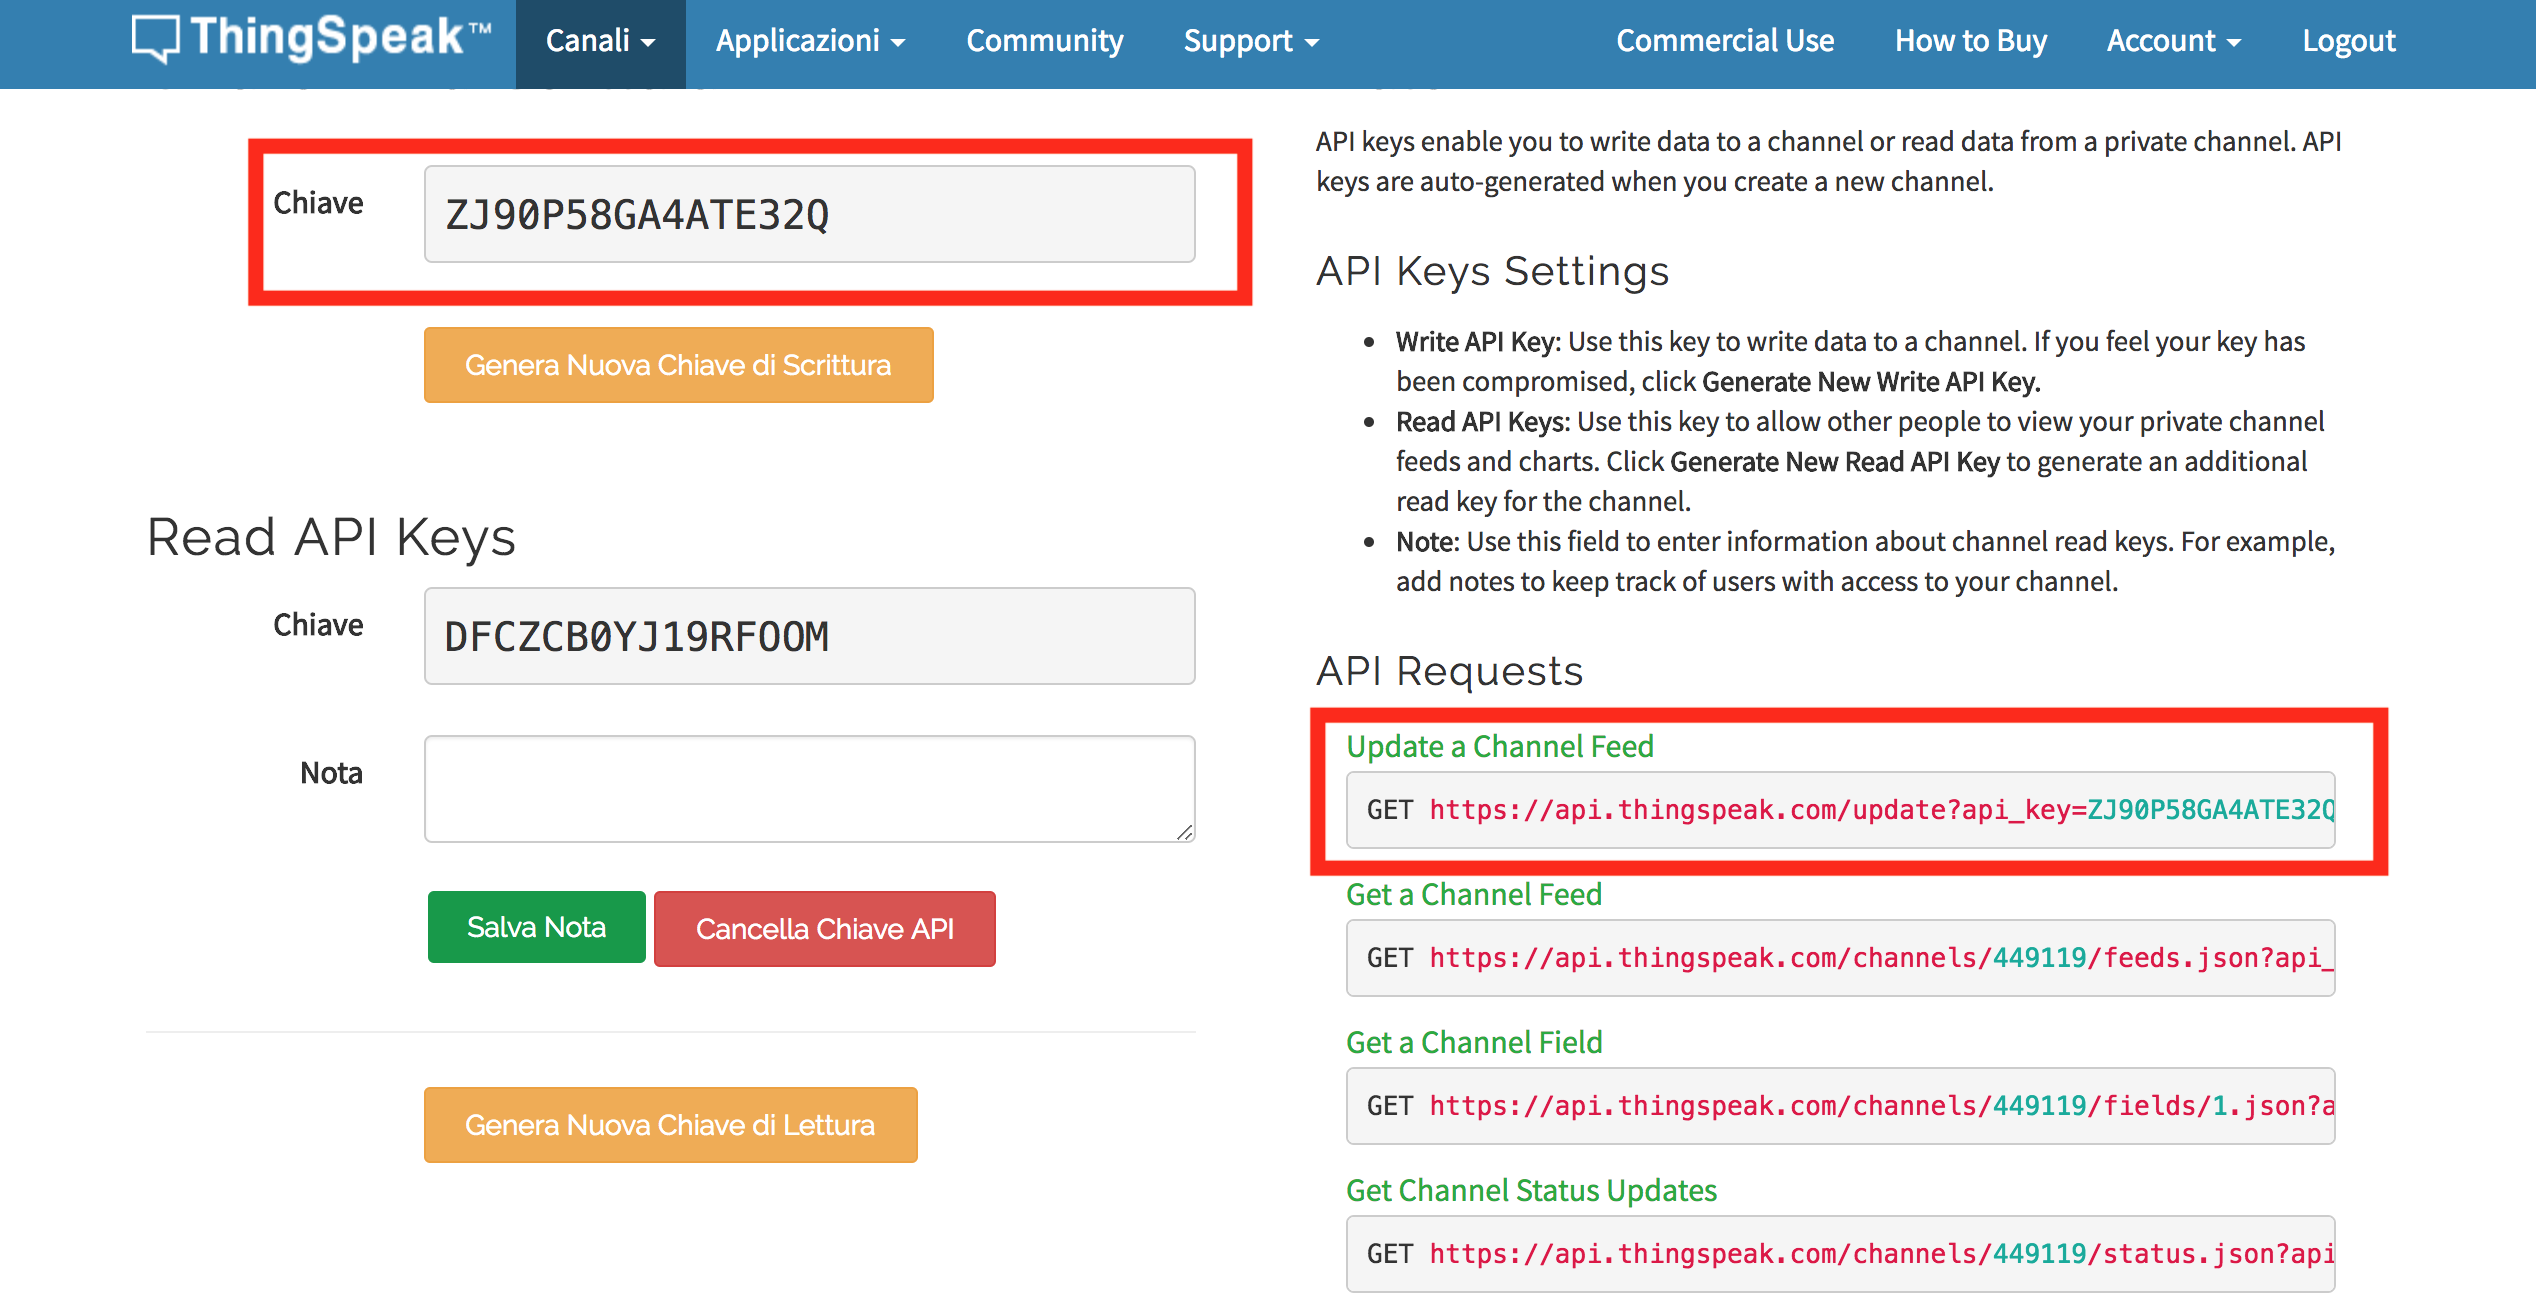
\includegraphics[width=0.8\textwidth]{./pictures/thingspeak-apis}
		\caption{ThingSpeak APIs}
		\label{mqtt_functioning}
	\end{center}
\end{figure}

\subsubsection{Node-RED communication}

The nodes used for the communication with ThingSpeak are the following
\begin{itemize}
    \item \textbf{FUNCTION}: taken from the function nodes menu. \\
    This node is used to setup the Http get request and indeed here we copy the write API Key of ThingSpeak.
    \item \textbf{HTTP REQUEST}: taken from the function nodes menu. \\
    This node is responsible to perform the Http get request towards ThingSpeak with the parameters passed from the function node.
\end{itemize}

\subsubsection{ThingSpeak Charts}
Once received some data samples, this is how ThingSpeak shows them.

\begin{figure}[H]
	\begin{center}
		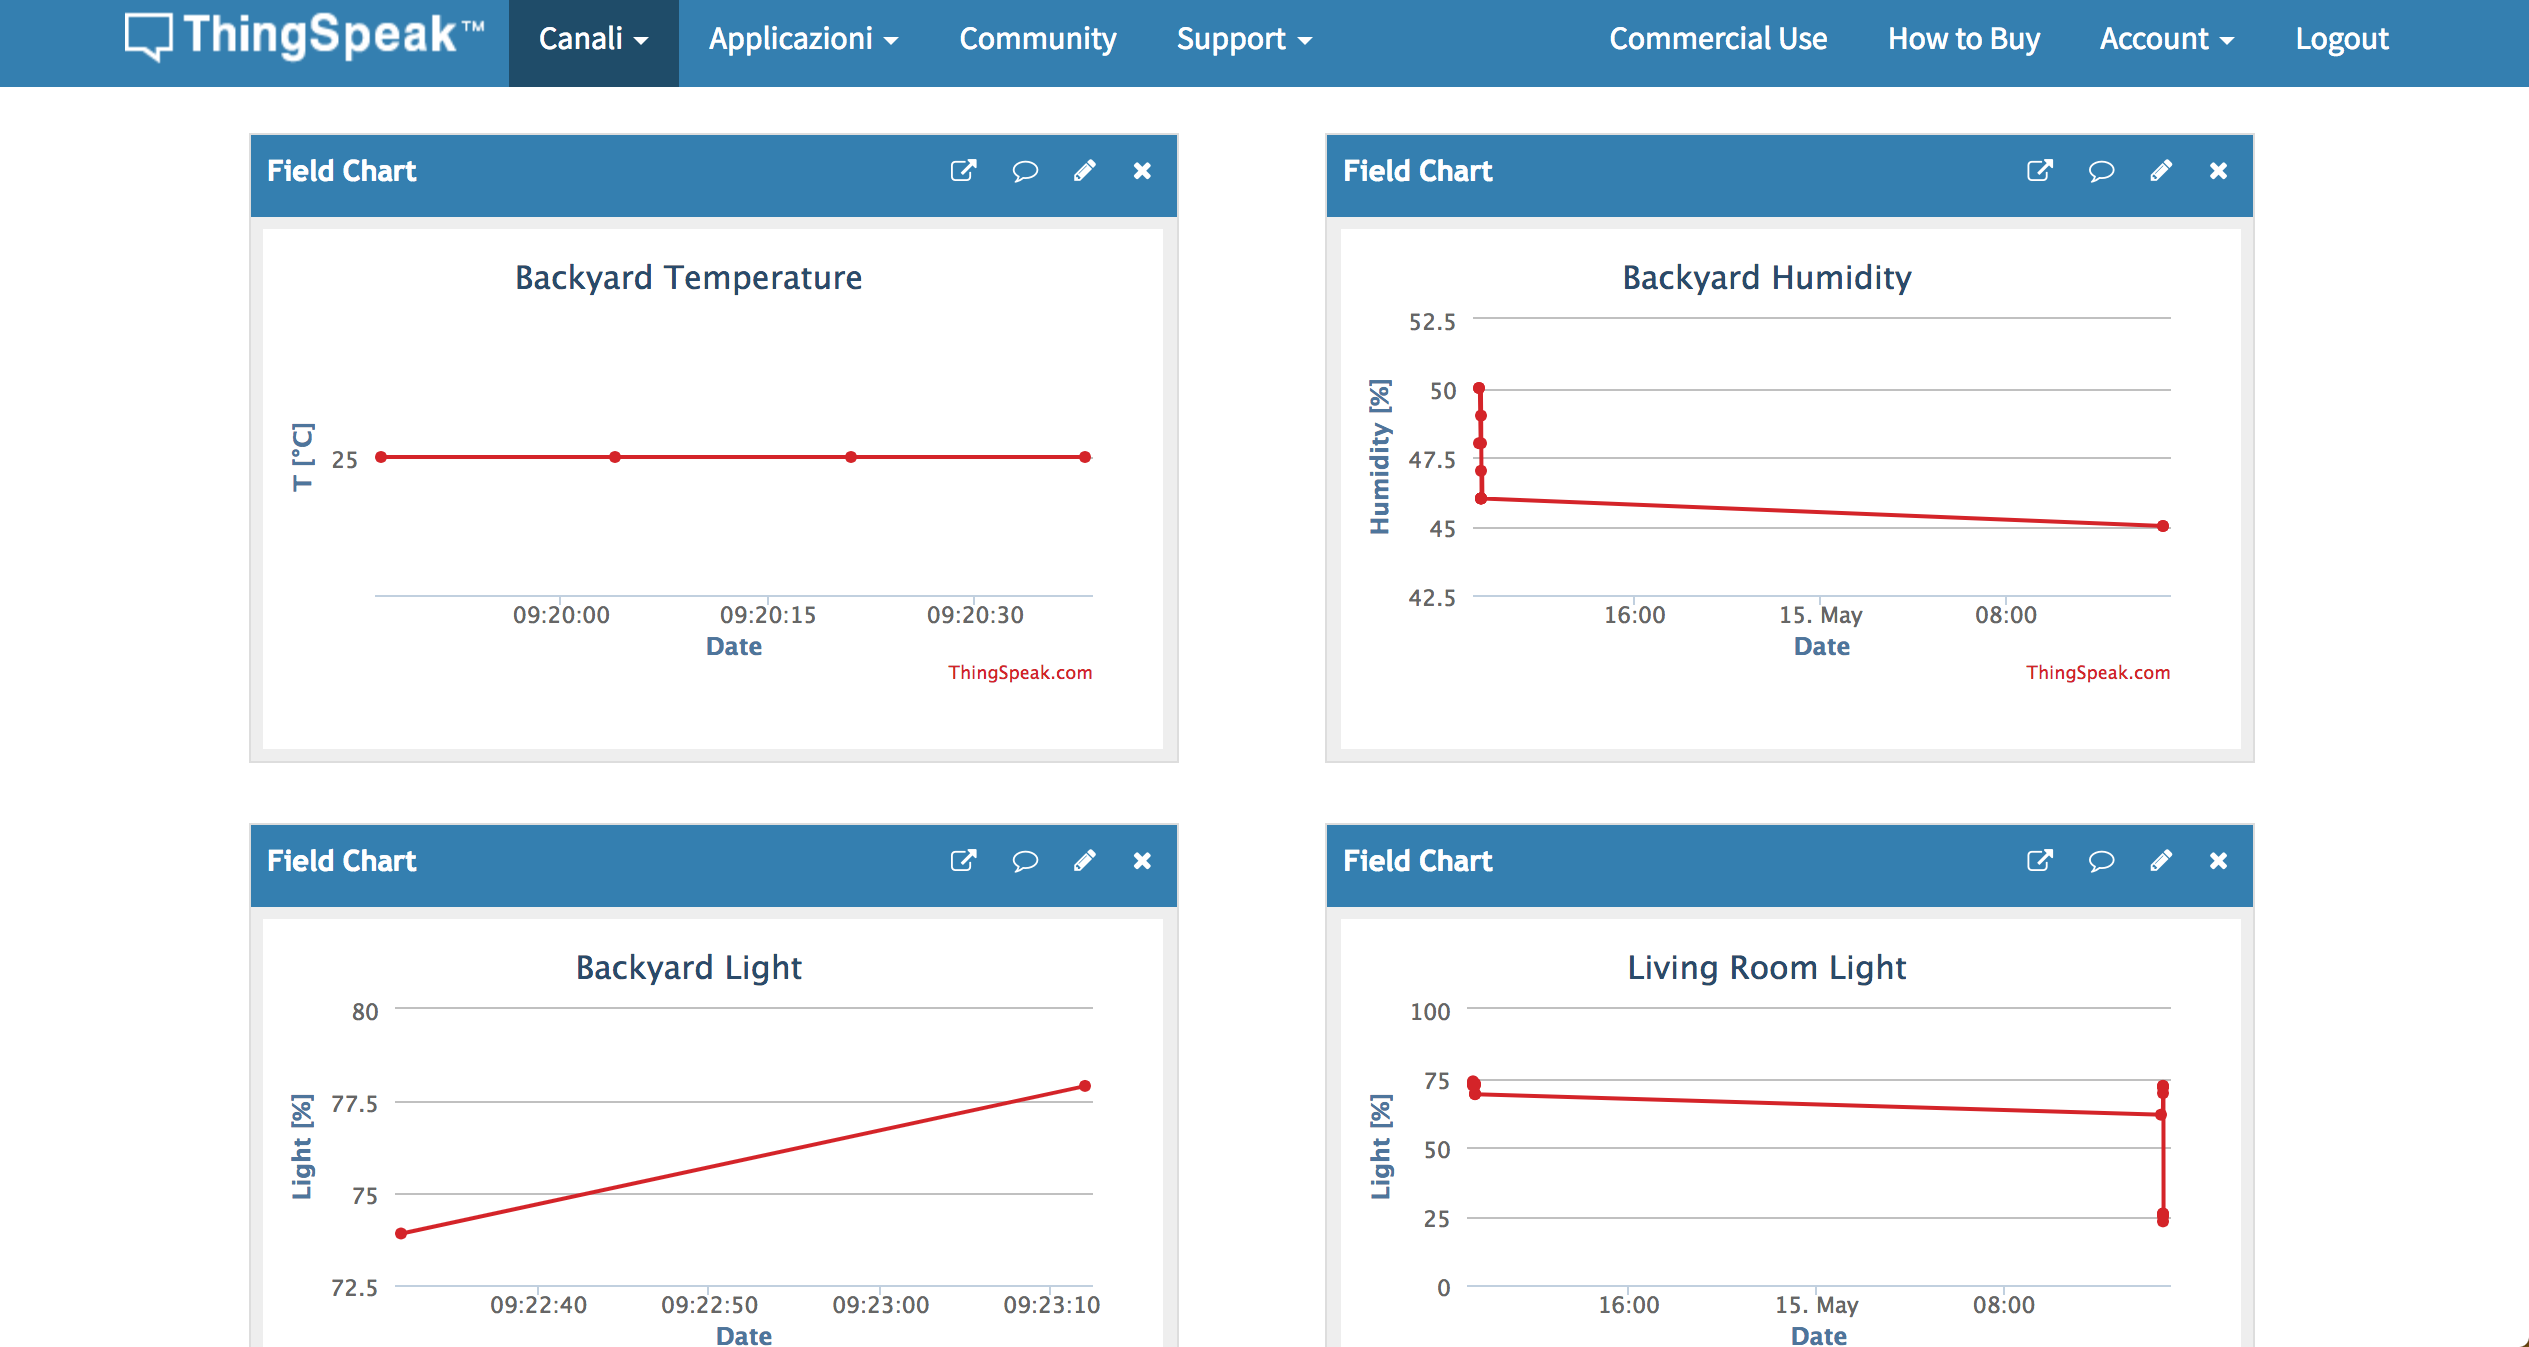
\includegraphics[width=0.8\textwidth]{./pictures/thingspeak-channel-charts}
		\caption{ThingSpeak Charts}
		\label{mqtt_functioning}
	\end{center}
\end{figure}
\section{Getting Started with ESP Boards}

% Schematici + commento codice
The \textit{Home Automation and Monitoring} system makes use of ESP modules to collect data from sensors and transmit them to the Raspberry Pi taking advantage of MQTT protocol.

Two kinds of boards have been selected to play the role of MQTT client; namely NodeMCU ESP-12E and ESP-32 development kits. The former is based on the widely explored ESP8266 System-On-Chip, which combines WiFi and microcontroller capabilities. The latter utilizes an ESP32 SoC that is very similar, but far more powerful: it has been designed to provide robustness, versatility and reliability in a wide variety of applications.

Both the boards can be easily programmed using the Arduino IDE after installing the appropriate cores via Arduino Boards Manager. The core installation will not be covered by this document.

Please notice that there is not a particular reason to use one specific board or the other: they both can fulfill the requirements of the system. The usage of different boards creates heterogeneity and variety, which are always present in the real world. 

\subsection{ESP-12E: Sensors, Wiring and Code}
\label{esp12_getting_started}
An accurate picture of the board pinout is shown in Figure \ref{esp12_pinout}. The ESP8266 module requires 3.3V power supply. Luckily the board provides a voltage regulator and can be connected to 5V using microUSB connector or \textit{Vin} pin.

\begin{figure}[H]
	\begin{center}
		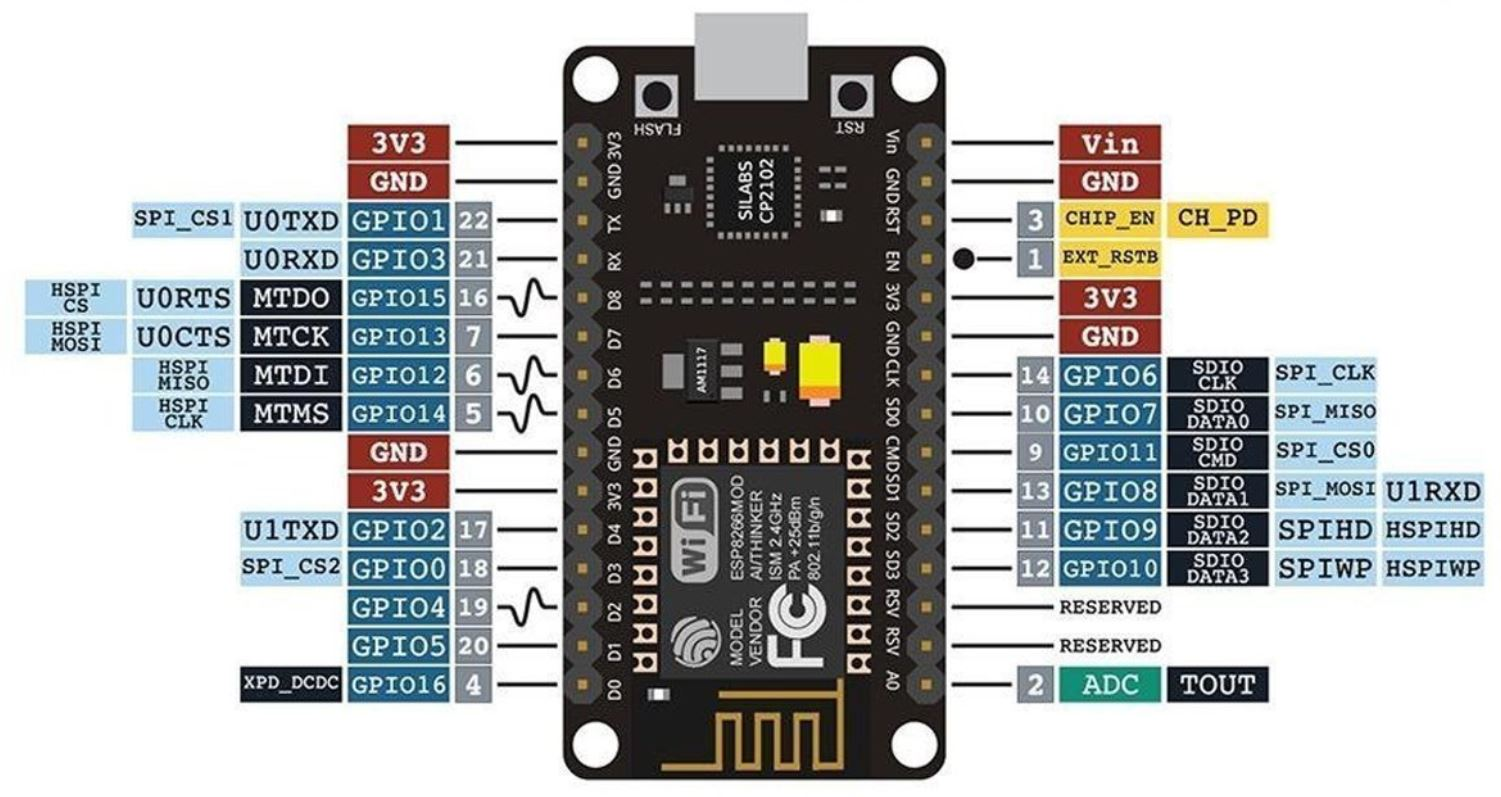
\includegraphics[width=\textwidth]{./pictures/ESP-12E_pinout.JPG}
		\caption{ESP-12E pinout.}
		\label{esp12_pinout}
	\end{center}
\end{figure}

\noindent
There is a number of two ESP-12E boards involved in the system. They both have the same configuration, sensors and wiring, but can be deployed in two different areas.
In more details, each board takes advantage of temperature, humidity and light sensors.

\subsubsection{Status LEDs}
Three LEDs give information about the status of the board:

\begin{itemize}
	\item \textbf{\textcolor{red}{Red}}: the board is trying to get WiFi access.
	\item \textbf{\textcolor[rgb]{1,0.8,0}{Yellow}}: the board is setting up MQTT connection. The MQTT broker must be up and running to succeed.
	\item \textbf{\textcolor[rgb]{0,0.6,0}{Green}}: the board is active and it is sending sensor data to the MQTT broker or listening to messages related to its subscriptions.
\end{itemize}

\subsubsection{Temperature and humidity sensor}
DHT11 and DTH22 are low cost temperature and humidity sensors. They are made of two parts: a thermistor and a capacitive humidity sensor. A small chip inside performs analog to digital conversion to let any microcontroller read the digital output signal.

Even though the two DHT sensors are interchangeable, DHT22 is more accurate and covers a larger range of temperatures.

Since the system involves two ESP-12E boards, both the sensors are used for the sake of completeness. Moreover, the fact that it is fairly easy to connect up to them, as shown in Figure \ref{esp12_wiring}, the low cost and ease of interfacing make these sensors an appropriate choice for the system.

\subsubsection{Light sensor}
A light sensor can be used to detect the current ambient light level, in particular the presence or absence of light. There exist several types of light sensors: photoresistors, phototransistors, photodiodes...

The chosen approach is making use of a photoresistor, taking advantage of the ADC provided by the ESP boards.

A photoresistor changes its resistance based on the amount of light that falls upon it: the more the light, the less the resistance. A simple voltage divider can be used to give an input to the ADC, as illustrated by Figure \ref{esp12_wiring}.

\subsubsection{Deep sleep}
ESP8266, the core of ESP-12E boards, supports sleeping. While sleeping, the device draws much less power than while awake: this could be a good approach to save power when batteries are the only source of electricity.

Deep sleep is one out of four supported types of sleep mode: everything is off but the Real Time Clock. This is the most power efficient option.

Pin D0 (GPIO 16) needs to be connected to RST to wake up the device when deep sleep is over: whenever RST receives a LOW signal, it restarts the microcontroller. Once the device is in deep sleep mode, a LOW signal will be sent to GPIO 16 as soon as the timer is up.

\begin{figure}[H]
	\begin{center}
		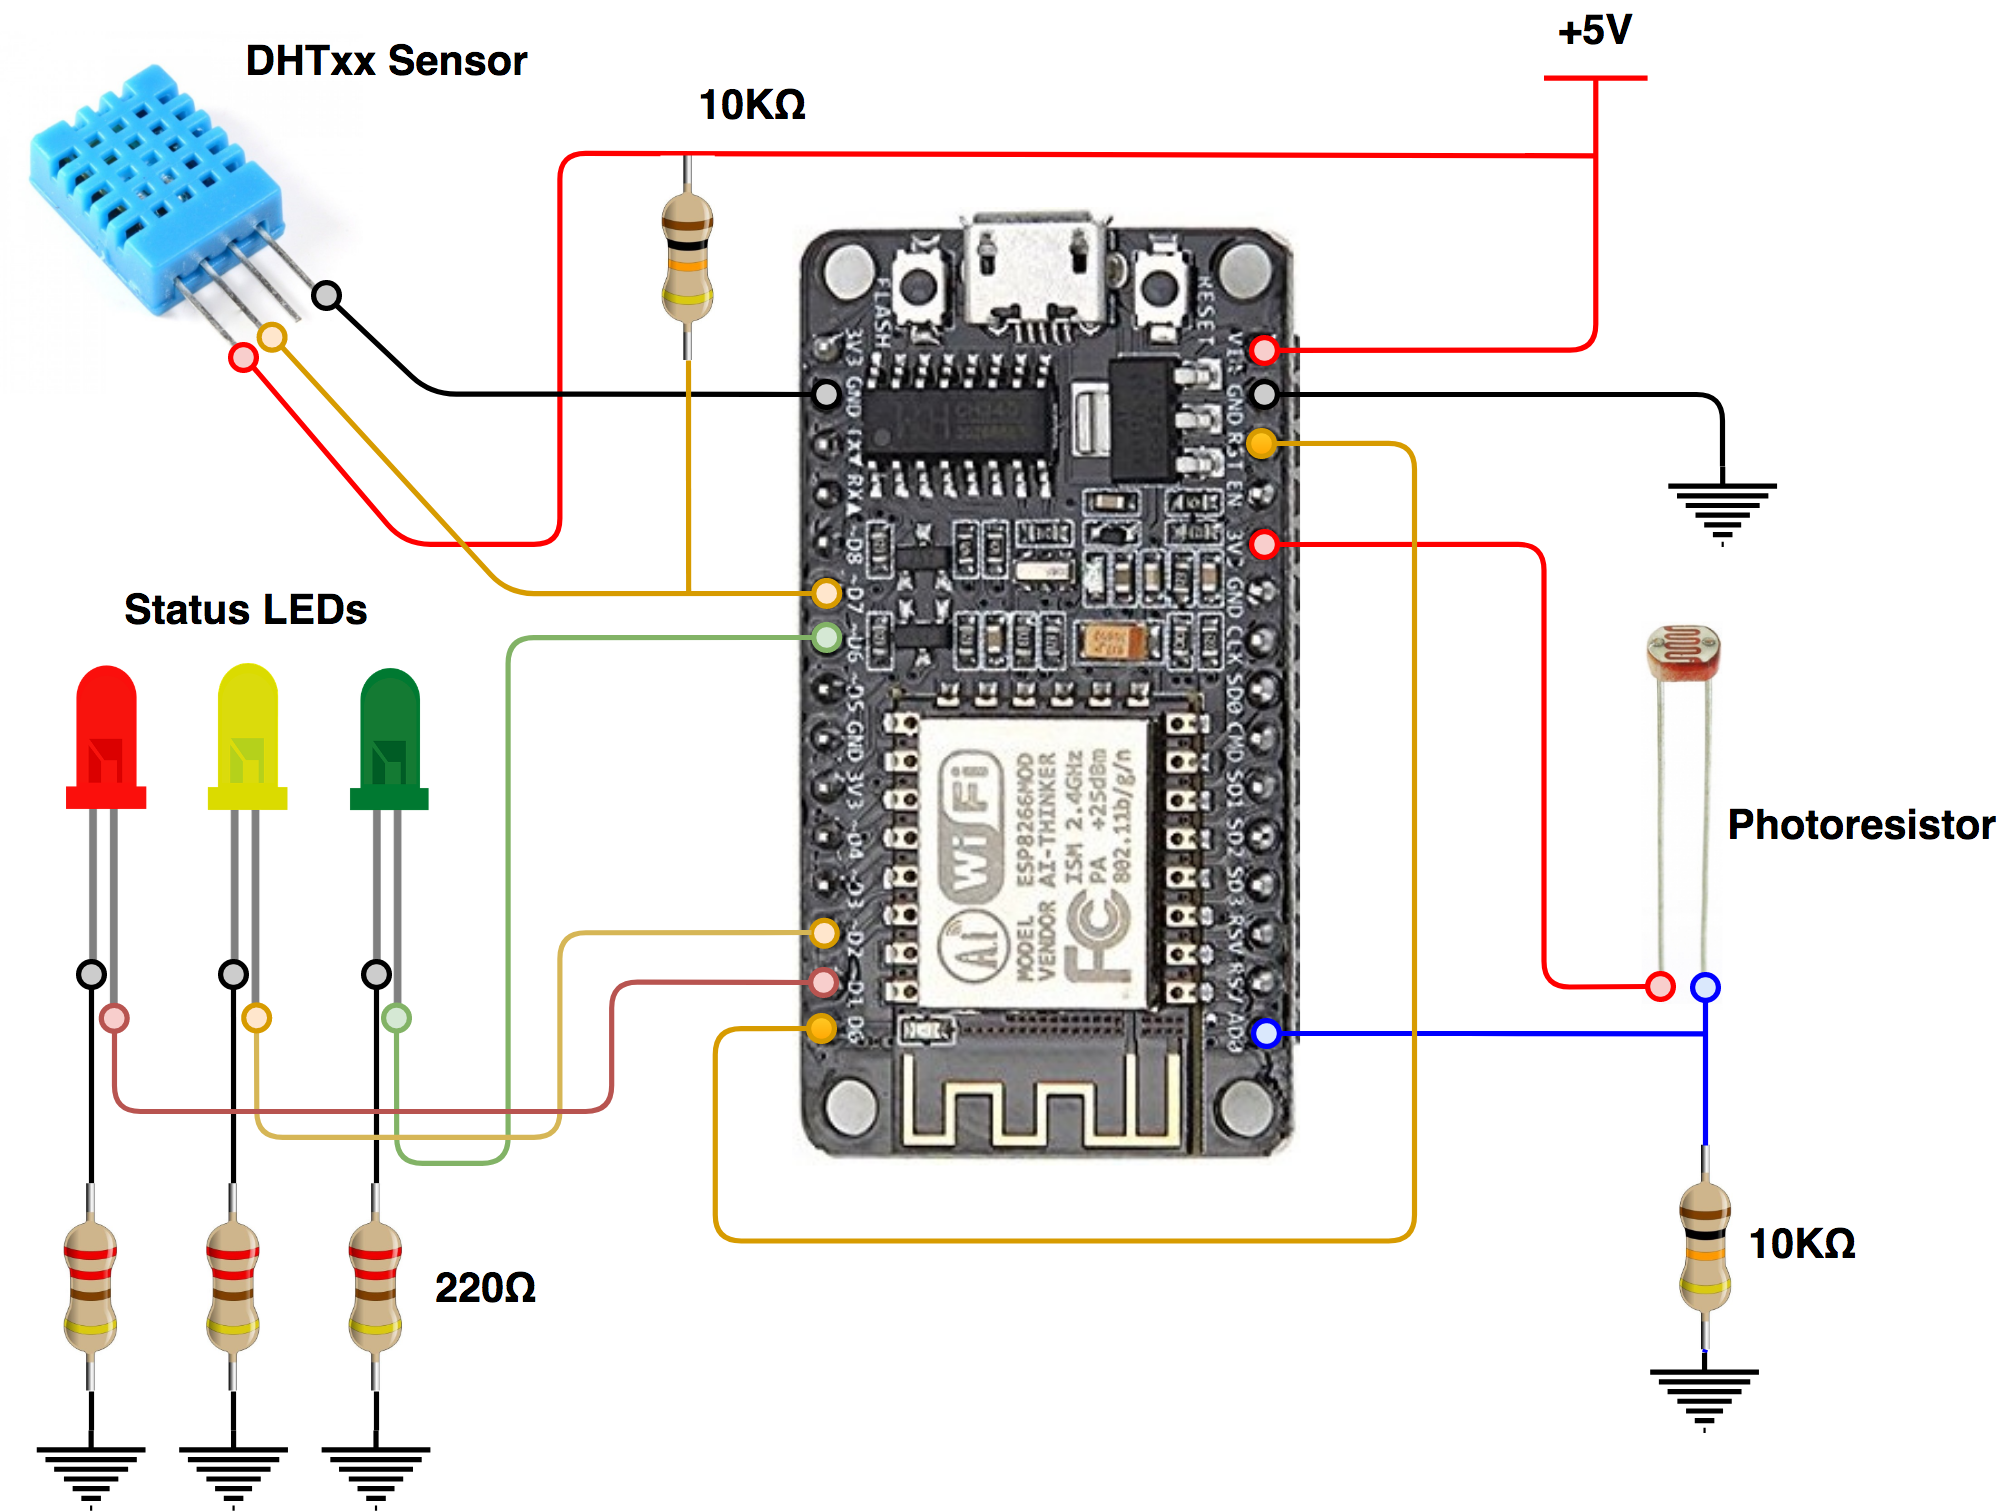
\includegraphics[width=\textwidth]{./pictures/ESP-12E_wiring.png}
		\caption{ESP-12E schematic with sensors and status LEDs. Notice the wire to tie D0 to RST pin to enable deep sleep.}
		\label{esp12_wiring}
	\end{center}
\end{figure}

\subsubsection{Code}
The main parts of the code are described by the following tables. In more detail, libraries are reported by Table \ref{esp12_code_libraries}, define preprocessor directives by Table \ref{esp12_code_defines}, global variables by Table \ref{esp12_global_variables} and, lastly, functions by Table \ref{esp12_functions}.

\noindent\begin{minipage}{\textwidth}
\begingroup
\setlength{\LTleft}{-20cm plus -1fill}
\setlength{\LTright}{\LTleft}
	\begin{longtable}{l | l}
		\hline
		\textbf{Library} & \textbf{Description} \\
		\hline
		\hline
		\texttt{ESP8266WiFi.h} & Required to enable WiFi connectivity. \\
		\hline
		\texttt{DHT.h} & Required to interface with DHT sensors. \\
		\hline
		\texttt{Adafruit\_MQTT.h} & Required to take advantage of MQTT protocol. \\ 
		\texttt{Adafruit\_MQTT\_Client.h} &  \\
		\hline

	\caption{Libraries involved in the sketches for ESP-12E boards.}
	\label{esp12_code_libraries}
	\end{longtable}
\endgroup
\end{minipage}

\noindent\begin{minipage}{\textwidth}
\begingroup
\setlength{\LTleft}{-20cm plus -1fill}
\setlength{\LTright}{\LTleft}
	\begin{longtable}{l | l}
		\hline
		\textbf{\#define Directive} & \textbf{Description} \\
		\hline
		\hline
		\texttt{DEBUG} & Enables debug over serial communication. \\
		\hline
		\texttt{WLAN\_SSID} & Name of the WiFi network to connect to. \\
		\texttt{WLAN\_PASS} & Password to join the WiFi network. \\ 
		\hline
		\texttt{HOST} & MQTT broker IP address. \\
		\texttt{PORT} & MQTT broker port. \\
		\texttt{USERNAME} & Credentials to set up the MQTT connection. \\
		\texttt{PASSWORD} & Credentials to set up the MQTT connection. \\
		\hline
		\texttt{SLEEP\_TIME}    & Deep sleep duration. \\
		\texttt{CONN\_ATTEMPTS} & Number of attempts to get WiFi connection \\
					            & before entering deep sleep mode. \\
		\texttt{MQTT\_ATTEMPTS} & Number of attempts to connect to MQTT service \\
		                        & provided by the broker. \\
		\hline
		\texttt{DHT\_TYPE} & Type of DHT sensor. \\
		\texttt{DHT\_PIN}  & Digital pin to read data coming from DHT sensor. \\
		\hline
		\texttt{LED\_RED}    & GPIO that controls the red led. \\
		\texttt{LED\_YELLOW} & GPIO in charge of controlling the yellow led. \\
		\texttt{LED\_GREEN} & GPIO that controls the green led. \\
		\hline

	\caption{Define directives specified in the sketches for ESP-12E boards.}
	\label{esp12_code_defines}
	\end{longtable}
\endgroup
\end{minipage}

\noindent\begin{minipage}{\textwidth}
	\begingroup
	\setlength{\LTleft}{-20cm plus -1fill}
	\setlength{\LTright}{\LTleft}
	\begin{longtable}{l | l}
		\hline
		\textbf{Global Variable} & \textbf{Description} \\
		\hline
		\hline
		\texttt{client} & This object is instantiated to enable WiFi connectivity. \\
		\hline
		\texttt{mqtt} & This object handles MQTT connection with the broker. \\
		\hline
		\texttt{temperature} & Objects of type Adafruit\_MQTT\_Publish in order to send \\ 
		\texttt{humidity}    & data to the broker. They are initialized with the appropriate \\
		\texttt{light}       & topic depending on the node that collects information.   \\
		\hline
		\texttt{dht} & Object that represent the DHT temperature and humidity sensor. \\
		             & It is instantiated specifying the type of sensor and the input pin \\
		             & on the board. \\
		\hline
		
		\caption{Global variables declared in the sketches for ESP-12E boards.}
		\label{esp12_global_variables}
	\end{longtable}
	\endgroup
\end{minipage}

\noindent\begin{minipage}{\textwidth}
	\begingroup
	\setlength{\LTleft}{-20cm plus -1fill}
	\setlength{\LTright}{\LTleft}
	\begin{longtable}{l | l}
		\hline
		\textbf{Function} & \textbf{Description} \\
		\hline
		\hline
		void \texttt{setup()} & Calls functions to establish WiFi connection and set up \\
							  & MQTT. It publishes data and enters deep sleep state. \\
		\hline
		void \texttt{loop()} & This function is not required since deep sleep is enabled. \\
						     & Every time the ESP-12E board restarts, the setup function is \\
		                     & executed and deep sleep state is entered. \\
		\hline
		void \texttt{enterDeepSleep()} & Turns off LEDs and WiFi and enters deep sleep state. \\
		\hline
		void \texttt{MQTT\_connect()} & Connects to MQTT service provided by the MQTT broker. \\
		\hline
		void \texttt{ledOff()} & Turns off the status LEDs.\\
		void \texttt{ledRed()} & Turns on the red LED.\\
		void \texttt{ledYellow()} & Turns on the yellow LED.\\
		void \texttt{ledGreen()} & Turns on the green LED.\\
		\hline
		
		\caption{Functions used in the sketches for ESP-12E boards.}
		\label{esp12_functions}
	\end{longtable}
	\endgroup
\end{minipage}

\subsection{ESP-32: Sensors, Wiring and Code}
An accurate picture of the board pinout is shown in Figure \ref{esp32_pinout}. As for ESP8266, also ESP32 requires 3.3V to operate. The board is provided with a voltage regulator and can be powered up by an external power source through USB connection or \textit{Vin} pin.

\begin{figure}[H]
	\begin{center}
		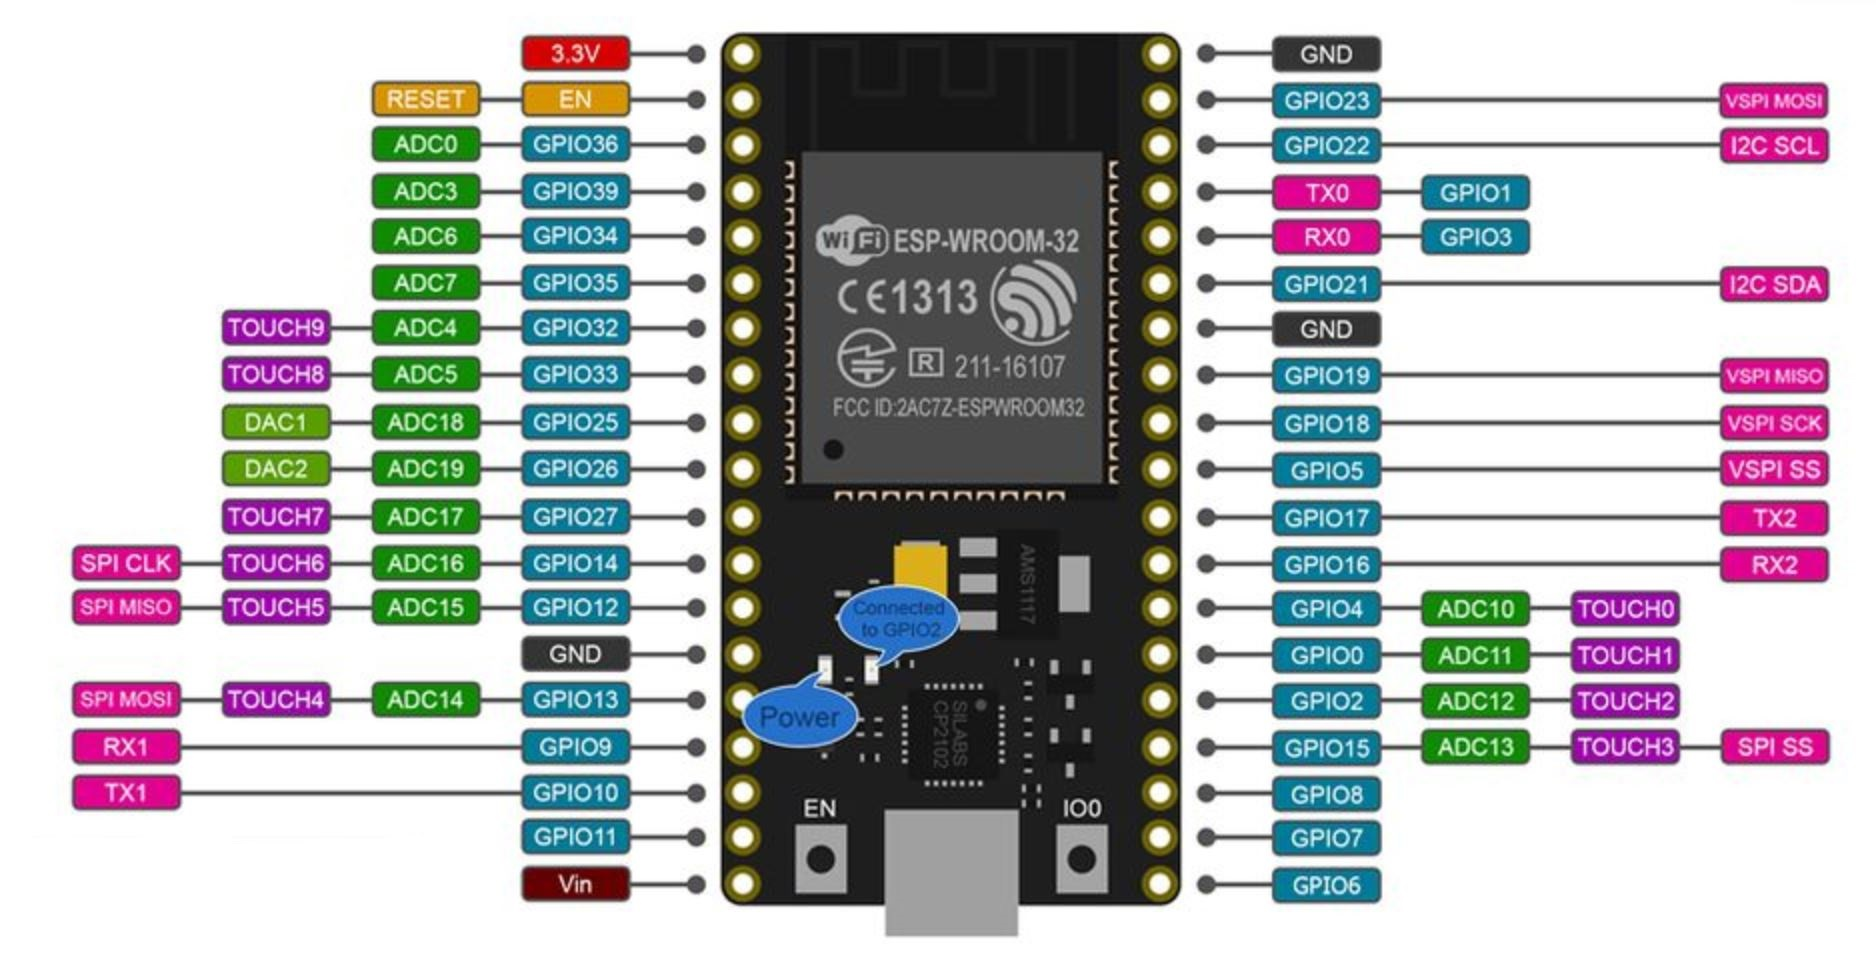
\includegraphics[width=\textwidth]{./pictures/ESP-32_pinout.JPG}
		\caption{ESP-32 pinout. Notice the presence of multiple ADC pins, in contrast with the only one offered by ESP-12E boards.}
		\label{esp32_pinout}
	\end{center}
\end{figure}

\noindent
Just a single board of this type is involved in the system. It is hooked up to a light sensor and to a relay module. The board does not take advantage of deep sleep functionality because it needs to be always up and running in order to reduce the latency to switch on and off the relay.

\subsubsection{Status LEDs}
Three LEDs fit out information about the status of the board. They work exactly as for ESP-12E boards: make reference to subsection \ref{esp12_getting_started}.

\subsubsection{Light sensor}
A photoresistor and a voltage divider are used to provide light intensity information. The operating principle is the same as for ESP-12E boards: please, make reference to subsection \ref{esp12_getting_started}.

\subsubsection{Relay module}
A relay is an electrical switch operated by an electromagnet. Relays are usually used to control a high voltage circuit with a low power one. A microcontroller can drive relays with one of its digital output pins: this is exactly what ESP32 is used for.

The advanced WiFi connectivity of the board gives the possibility to remotely control the digital pin hooked to the relay module turning it into a remote switch.

As mentioned earlier, in order to reduce the latency to turn on and off the relay, the module is always active and does not enter any sleep state.

\begin{figure}[H]
	\begin{center}
		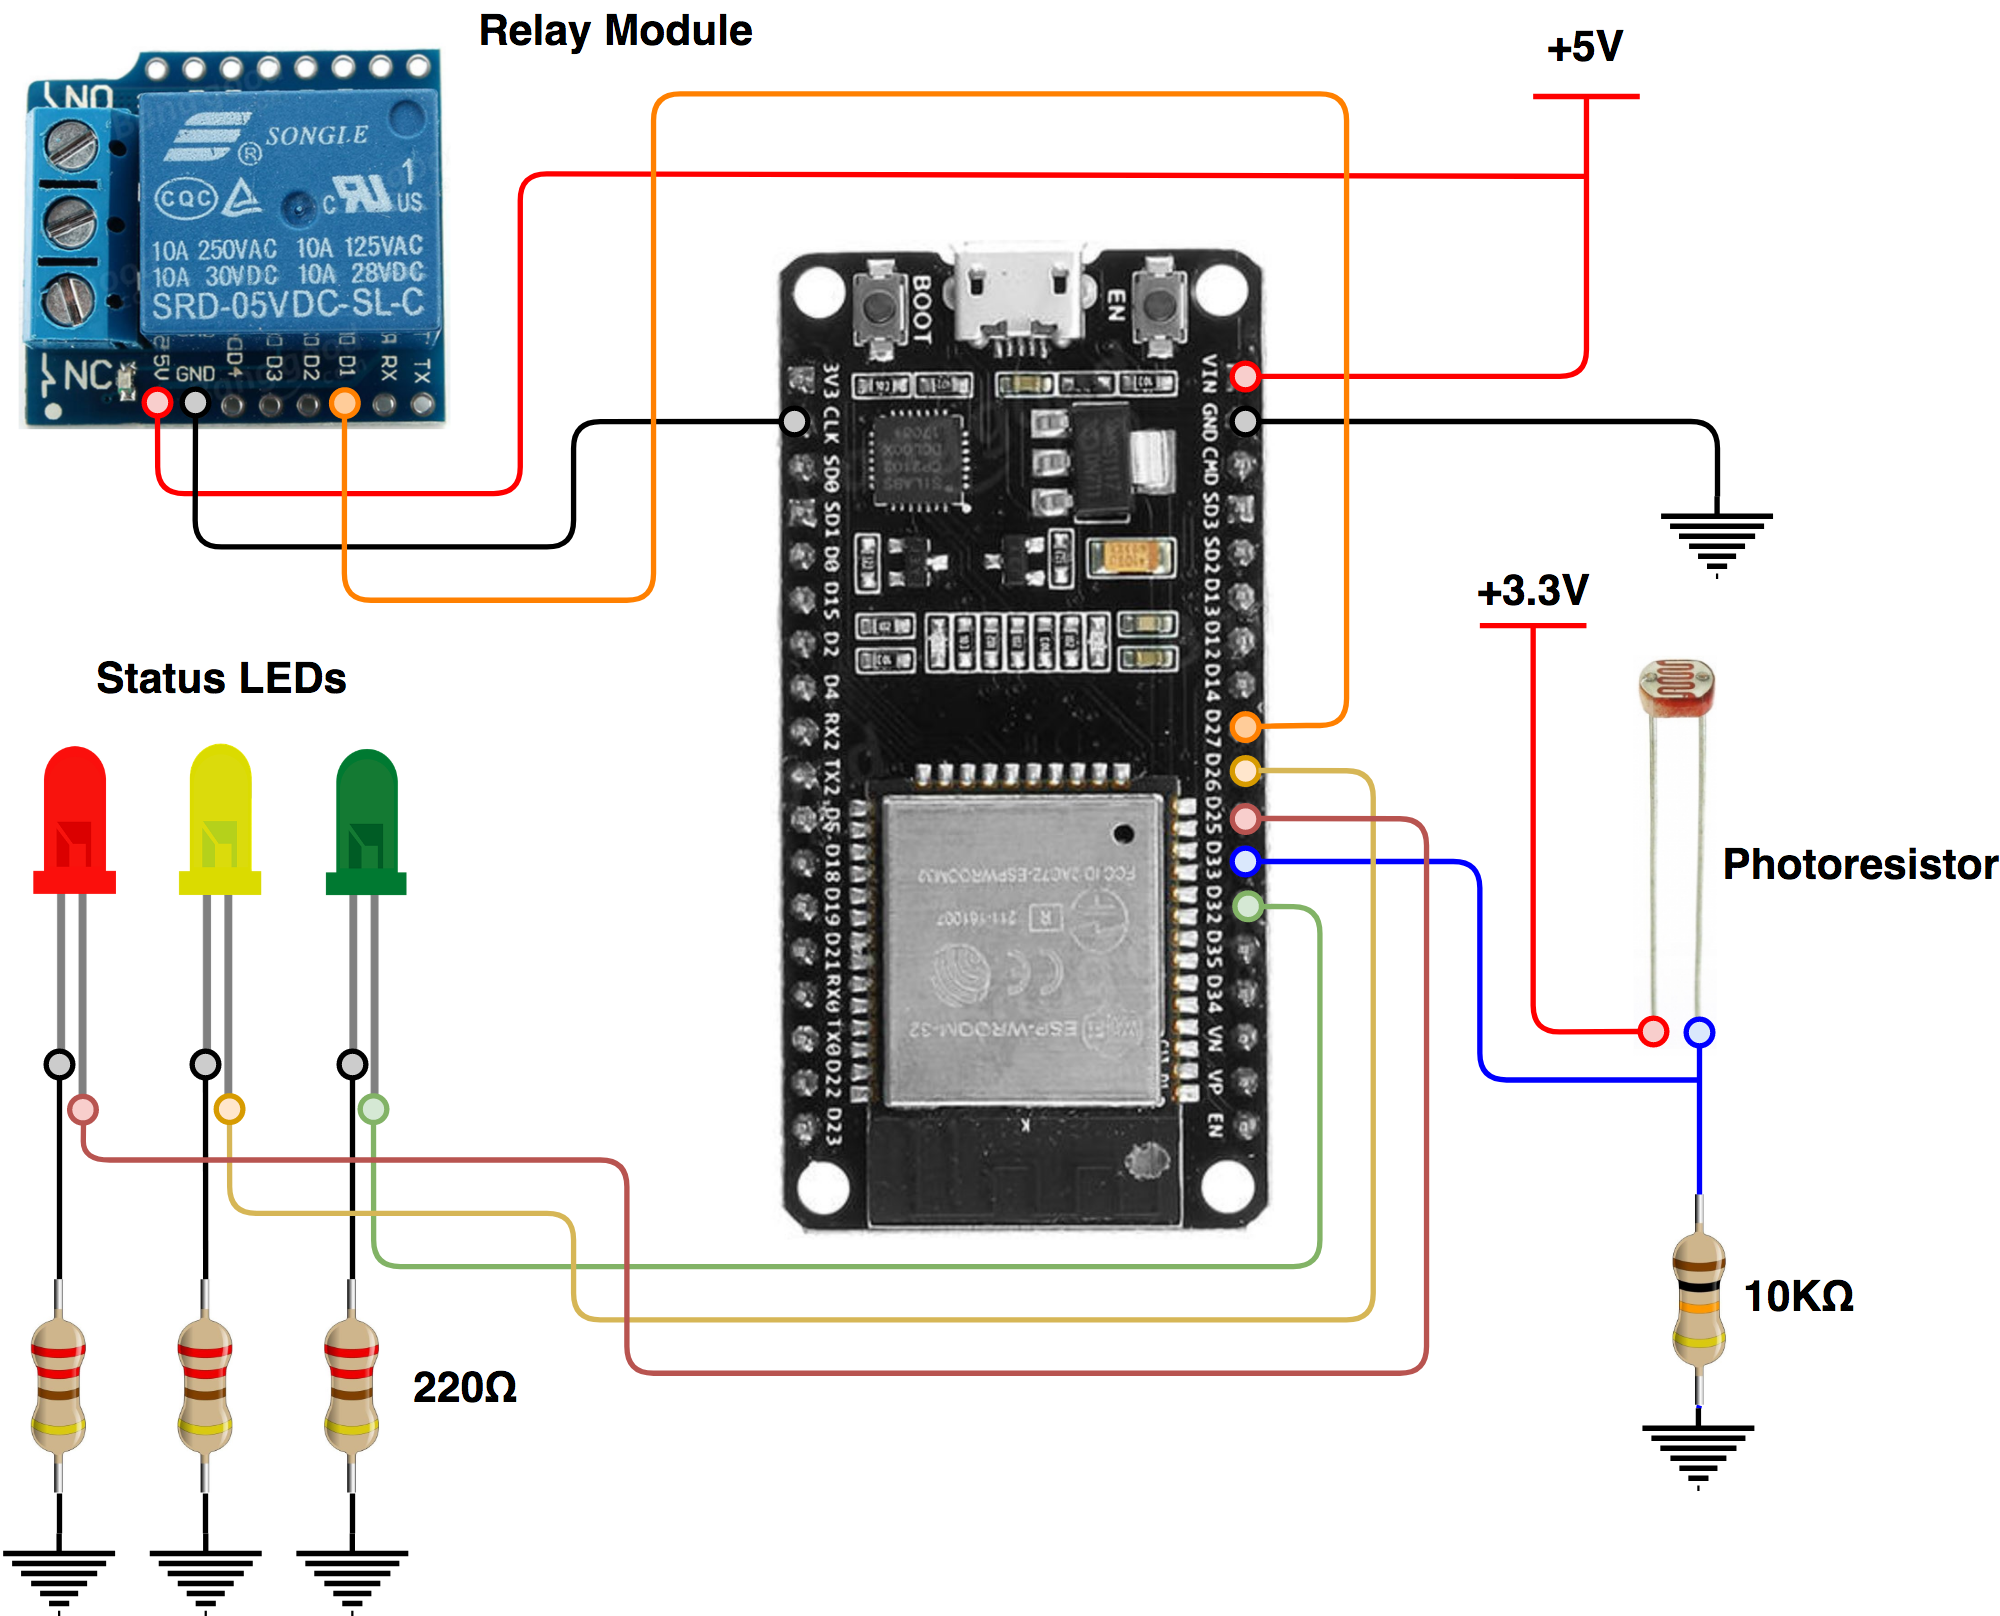
\includegraphics[width=\textwidth]{./pictures/ESP-32_wiring.png}
		\caption{ESP-32 schematic with sensors, actuators and status LEDs.}
		\label{esp32_wiring}
	\end{center}
\end{figure}

\subsubsection{Code}
As for ESP-12 boards, the main parts of the code are described by the following tables. In more detail, libraries are reported by Table \ref{esp32_code_libraries}, define preprocessor directives by Table \ref{esp32_code_defines}, global variables by Table \ref{esp32_global_variables} and, lastly, functions by Table \ref{esp32_functions}.

\noindent\begin{minipage}{\textwidth}
	\begingroup
	\setlength{\LTleft}{-20cm plus -1fill}
	\setlength{\LTright}{\LTleft}
	\begin{longtable}{l | l}
		\hline
		\textbf{Library} & \textbf{Description} \\
		\hline
		\hline
		\texttt{WiFi.h} & Required to enable WiFi connectivity. \\
		\hline
		\texttt{Adafruit\_MQTT.h} & Required to deal with MQTT protocol. \\ 
		\texttt{Adafruit\_MQTT\_Client.h} & \\
		\hline
		
		\caption{Libraries involved in the sketch for ESP-32 board.}
		\label{esp32_code_libraries}
	\end{longtable}
	\endgroup
\end{minipage}

\noindent\begin{minipage}{\textwidth}
	\begingroup
	\setlength{\LTleft}{-20cm plus -1fill}
	\setlength{\LTright}{\LTleft}
	\begin{longtable}{l | l}
		\hline
		\textbf{\#define Directive} & \textbf{Description} \\
		\hline
		\hline
		\texttt{DEBUG} & Enables debug over serial communication. \\
		\hline
		\texttt{WLAN\_SSID} & Name of the WiFi network to connect to. \\
		\texttt{WLAN\_PASS} & Password to join the WiFi network. \\ 
		\hline
		\texttt{HOST} & MQTT broker IP address. \\
		\texttt{PORT} & MQTT broker port. \\
		\texttt{USERNAME} & Credentials to set up the MQTT connection. \\
		\texttt{PASSWORD} & Credentials to set up the MQTT connection. \\
		\hline
		\texttt{LED\_RED}    & GPIO that controls the red led. \\
		\texttt{LED\_YELLOW} & GPIO in charge of controlling the yellow led. \\
		\texttt{LED\_GREEN} & GPIO that controls the green led. \\
		\hline
		\texttt{LIGHT\_ADC} & GPIO that provides ADC functionality to sample the \\
							& analog voltage coming from the photoresistor. \\
		\hline
		\texttt{SWITCH\_PIN} & GPIO to switch on and off the relay module. \\
		\hline
		\texttt{WAIT\_TIME} & Interval of time to listen to subscription messages. \\
		\hline
		
		\caption{Define directives specified in the sketch for ESP-32 board.}
		\label{esp32_code_defines}
	\end{longtable}
	\endgroup
\end{minipage}

\noindent\begin{minipage}{\textwidth}
	\begingroup
	\setlength{\LTleft}{-20cm plus -1fill}
	\setlength{\LTright}{\LTleft}
	\begin{longtable}{l | l}
		\hline
		\textbf{Global Variable} & \textbf{Description} \\
		\hline
		\hline
		\texttt{client} & This object is instantiated to enable WiFi connectivity. \\
		\hline
		\texttt{mqtt} & This object handles MQTT connection with the broker. \\
		\hline
		\texttt{light} & Object of type Adafruit\_MQTT\_Publish in order to send \\
					   & light intensity data to the broker. \\
		\hline
		\texttt{toggle\_switch} & Object of type Adafruit\_MQTT\_Subscribe to listen to \\
								& MQTT messages to enable and disable the relay module. \\
		\hline
		\texttt{sw\_status} & Keeps the status of the relay module. \\
		\hline
		
		\caption{Global variables declared in the sketch for ESP-32 board.}
		\label{esp32_global_variables}
	\end{longtable}
	\endgroup
\end{minipage}

\noindent\begin{minipage}{\textwidth}
	\begingroup
	\setlength{\LTleft}{-20cm plus -1fill}
	\setlength{\LTright}{\LTleft}
	\begin{longtable}{l | l}
		\hline
		\textbf{Function} & \textbf{Description} \\
		\hline
		\hline
		void \texttt{setup()} & Calls functions to establish WiFi connection and set up MQTT. \\
		\hline
		void \texttt{loop()} & Publishes data about light intensity and listens to messages \\
							 & related to the relay status for WAIT\_TIME milliseconds. \\
		\hline
		void \texttt{MQTT\_connect()} & Connects to MQTT service provided by the MQTT broker. \\
		\hline
		void \texttt{toggleSwitch()} & Flips the status (active/inactive) of the relay module. \\
		\hline
		void \texttt{ledOff()} & Turns off the status LEDs.\\
		void \texttt{ledRed()} & Turns on the red LED.\\
		void \texttt{ledYellow()} & Turns on the yellow LED.\\
		void \texttt{ledGreen()} & Turns on the green LED.\\
		\hline
		
		\caption{Functions used in the sketch for ESP-32 board.}
		\label{esp32_functions}
	\end{longtable}
	\endgroup
\end{minipage}